% =====================================================================
%  随机信号分析（第5版）  第2章 随机信号
%  由图片型 PDF 扫描件转录重排为 LaTeX 源码
%  编译：xelatex  （必须用 XeLaTeX/LuaLaTeX；pdflatex 无法处理中文）
%        xelatex -output-directory=<build> SSA_Textbook_CH2_zh.tex   （跑四遍，目录收敛）
%
%  ★ 主文件在 \chapter 之前必须有 \setcounter{chapter}{1}
%    否则公式会编成 (1.x)、图会编成 图1.x（原书应为 2.x）。
%    分片单独试编译时同样要设这个计数器。
% =====================================================================
\documentclass[11pt,openany,UTF8]{ctexbook}

% ---------- 页面：还原原书 168mm x 255mm 开本 ----------
\usepackage[%
  paperwidth=168mm,paperheight=255mm,
  top=20mm,bottom=18mm,inner=20mm,outer=16mm,
  headsep=5mm,footskip=8mm]{geometry}

% ---------- 数学 ----------
\usepackage{amsmath,amssymb,amsfonts,mathrsfs}
\usepackage{bm}

% ---------- 图表 ----------
\usepackage{graphicx}
\usepackage{tikz}
\usetikzlibrary{patterns,arrows.meta,positioning,calc}
\usepackage{wrapfig}
\usepackage{booktabs}
\usepackage{array}
\usepackage{multirow}  % 表2.1 里"随机函数集合/随机变量集合"两列纵向合并
\usepackage{diagbox}   % 斜线表头（如习题里的联合分布律表\nobreak）
\usepackage{tcolorbox}
\tcbuselibrary{skins,breakable}

% ---------- 其它 ----------
\usepackage{fancyhdr}
\usepackage[hidelinks]{hyperref}
\hypersetup{
  pdftitle={随机信号分析（第5版\nobreak）第2章 随机信号},
  pdfauthor={李晓峰 等},
  pdfsubject={Stochastic Signal Analysis, Glasgow College UESTC},
  pdfkeywords={随机信号, 随机过程, 随机正弦信号, 伯努利随机序列, 半随机二进制传输信号, 泊松过程, 高斯信号, 独立信号},
}

% 绕排图形会压缩行宽，留一点弹性，避免字间距被拉得过开
\setlength{\emergencystretch}{1.5em}

% 图/表题注：统一用 caption 宏包。原书为「图1.1 题注」式，无冒号。
% \captionof{figure}{...} 用于不能放浮动体的场合（例如灰底例题框内部）。
\usepackage{caption}
\captionsetup{labelsep=quad,skip=3pt,font=small}

% 插图浮动参数：原书图随文走，这里放宽约束，避免图被推到单独一页、
% 或与正文引用处相隔过远。
\setcounter{topnumber}{3}
\setcounter{bottomnumber}{2}
\setcounter{totalnumber}{4}
\renewcommand{\topfraction}{0.92}
\renewcommand{\bottomfraction}{0.85}
\renewcommand{\textfraction}{0.06}
\renewcommand{\floatpagefraction}{0.55}
\setlength{\floatsep}{8pt plus 2pt minus 2pt}
\setlength{\textfloatsep}{10pt plus 2pt minus 2pt}
\setlength{\intextsep}{8pt plus 2pt minus 2pt}

% =====================================================================
%  关键修补：①②③…（U+2460–U+24FF 带圈数字）不在 xeCJK 默认 CJK 区段内，
%  若不声明，xeCJK 会把它们交给 Latin 字体（lmroman）而导致缺字空白。
% =====================================================================
\xeCJKDeclareCharClass{CJK}{"2460 -> "24FF, "3000 -> "303F, "FF00 -> "FFEF}

% =====================================================================
%  全书统一符号宏（保证 36 页公式风格一致，也便于日后统一修改）
% =====================================================================
\newcommand{\dif}{\mathrm{d}}                      % 微分算子 d
\newcommand{\eu}{\mathrm{e}}                       % 自然对数底 e
\newcommand{\ju}{\mathrm{j}}                       % 虚数单位 j
\newcommand{\E}{E}                                 % 数学期望（原书用斜体 E\nobreak）
\DeclareMathOperator{\Var}{Var}                    % 方差（原书亦写作 D(X)\nobreak，本文统一用 Var\nobreak）
\DeclareMathOperator{\Cov}{Cov}                    % 协方差
\DeclareMathOperator{\sgn}{sgn}
\newcommand{\R}{\mathbb{R}}                        % 实数集
\newcommand{\bX}{\bm{X}}
\newcommand{\bx}{\bm{x}}

% 原书正文里 1. / 2. / 3. 这类手工小标题（不进入自动编号）
\newcommand{\bhead}[1]{\par\medskip\noindent\textbf{#1}\par\smallskip}

% 定理/定义等着重标签。原书为「定义 2.1  设…」——标签与正文同一行，
% 故此处只另起一段，不强制折行（与 \bhead 的区别就在这里）。
\newcommand{\thm}[1]{\par\medskip\noindent\textbf{#1}\quad}

% 原书 ①②③ 式条目列表（保持悬挂缩进）
\newenvironment{citemize}
  {\begin{list}{}{\leftmargin=2.4em\itemindent=-2.4em\itemsep=1pt\topsep=3pt\parsep=0pt}}
  {\end{list}}

% ---------- 习题部分（书 p.61–62） ----------
% 习题标题：原书为居中加粗，并计入目录
\newcommand{\exhead}[1]{%
  \par\addvspace{1.6em}%
  \addcontentsline{toc}{section}{#1}%
  \centerline{\textbf{\zihao{4}#1}}%
  \par\addvspace{0.9em}}
% 单道习题：题号常规字重、另起一段（原书如此）
\newcommand{\exer}[1]{\par\medskip\noindent #1\quad\ignorespaces}
% 子问题两列排（原书：(1)(2) 一行，(3)(4) 一行）
\newenvironment{subq}
  {\par\smallskip\noindent
   \begin{tabular}{@{}p{0.465\linewidth}@{\hspace{0.05\linewidth}}p{0.465\linewidth}@{}}}
  {\end{tabular}\par}

% 例题盒子（原书为灰底方框，可跨页断行）
\newtcolorbox{examplebox}[1][]{
  colback=black!6, colframe=black!6, boxrule=0pt,
  left=3mm,right=3mm,top=2.5mm,bottom=2.5mm,
  breakable, #1}

% 页脚：还原原书 “· 页码 ·” 样式
\pagestyle{fancy}
\fancyhf{}
\fancyfoot[C]{\small\textperiodcentered\ \thepage\ \textperiodcentered}
\renewcommand{\headrulewidth}{0pt}

\ctexset{
  chapter/number={\arabic{chapter}},
  chapter/name={第,章},
  chapter/format=\centering\bfseries\zihao{3},
  chapter/beforeskip=12pt,
  chapter/afterskip=20pt,
  section/format=\bfseries\zihao{4},
  subsection/format=\bfseries\zihao{-4},
}

% =====================================================================

\begin{document}

% ====================== 封面 ======================
\begin{titlepage}
  \centering
  \vspace*{2.6cm}
  {\zihao{2}\bfseries 随机信号分析（第5版\nobreak）\par}
  \vspace{1.0cm}
  {\zihao{3}\bfseries 第2章\quad 随机信号\par}
  \vspace{0.5cm}
  {\zihao{4} 2.1–2.5 节\quad 附\quad 习题\par}
  \vspace{1.1cm}
  \rule{0.5\textwidth}{0.6pt}\par
  \vspace{1.1cm}
  {\zihao{4} 李晓峰\quad 等\par}
  \vfill
  {\zihao{5} Stochastic Signal Analysis\par}
  \vspace{0.25cm}
  {\zihao{5} Glasgow College, UESTC\par}
  \vspace{1.2cm}
  {\zihao{-5} 重排版\quad\textperiodcentered\quad 矢量可搜索 PDF\par}
  \vspace{1.6cm}
\end{titlepage}

% ====================== 目录 ======================
\tableofcontents
\thispagestyle{empty}
\clearpage
\setcounter{page}{1}

\setcounter{chapter}{1}
\chapter{随机信号}

% =====================================================================
%  frag_A —— 书 p.37–39（PDF p.51–53）
%  内容：章首引言、2.1 定义与基本特性、2.1.1 概念与定义、
%        2.1.2 基本概率特性（起）
%  本片编号：图2.1–2.4、表2.1、例2.1–2.3、定义2.1–2.2；无编号公式
%  接缝：本片结尾停在"描述随机信"处，句子后半截（"号的特性可以通过描述带 $t$ 的
%        随机变量 $X(t,\xi)$ 来实现。"）由 frag_B 从 p.40 第一行接着写。
% =====================================================================

在信号分析中\nobreak，我们把携带某种信息\nobreak、随时间\nobreak、空间或其他某个参量变化的物理量抽象为信号\nobreak，并使用确定的时间函数来表示它们\nobreak，例如\nobreak，$f(t)$ 或 $s(t)$\nobreak，这类信号是确定信号\nobreak。另外一大类信号源自于不确定的随机现象\nobreak，因而是随机的\nobreak，它们的特性服从某种统计规律\nobreak，该类信号称为随机信号\nobreak。

本章介绍随机信号的定义\nobreak、基本特性与描述方式\nobreak；讨论几个典型的信号例子及其基本的分析方法\nobreak；本章还介绍十分重要的高斯信号与独立信号\nobreak。

\section{定义与基本特性}
实际应用中的许多物理量既是按时间（或其他参量\nobreak）推进的\nobreak，又是随机的\nobreak，描述这类现象需要随机过程或随机信号\nobreak。

\subsection{概念与定义}
我们首先通过两个例子来考察一类随机现象\nobreak。

\begin{examplebox}
\textbf{例2.1}\quad 噪声电压信号\nobreak。电子设备中\nobreak，电阻上的噪声电压是典型的随机信号\nobreak。由于热电子的骚动\nobreak，引起电阻两端的电压有一个不确定的起伏\nobreak。对该电压进行一次观测可能记录到一段波形 $x_1(t)$\nobreak，而进行第二次观测又记录到一段不同的波形 $x_2(t)$\nobreak，$\cdots$\nobreak，如图~\ref{fig:2.1} 所示\nobreak。每次观测前我们都无法预知可能会记录到什么样的波形\nobreak，该电压信号是无穷多种可能波形中的某一个\nobreak。可见\nobreak，噪声电压信号是一族随机的函数\nobreak。

\begin{center}
  \begin{tikzpicture}[x=1cm,y=0.95cm,every node/.style={font=\small}]
    % ---------- (a) 第一次记录的波形 ----------
    \begin{scope}
      \draw[->] (0,0) -- (2.95,0);
      \node[below left] at (2.95,0) {$t$};
      \draw[->] (0,0) -- (0,1.28);
      \node[above] at (0,1.28) {$x_1(t)$};
      \node[below left] at (0.05,0.02) {$O$};
      \draw[thick] plot[samples=500,domain=0:2.55]
        (\x,{0.42+0.30*sin(deg(26*\x))*(0.62+0.38*sin(deg(1.1*\x+0.6)))+0.055*sin(deg(53*\x+1.3))});
      \node at (1.45,-0.70) {\small (a) 第一次记录的波形};
    \end{scope}
    % ---------- (b) 第二次记录的波形 ----------
    \begin{scope}[shift={(4.25,0)}]
      \draw[->] (0,0) -- (2.95,0);
      \node[below left] at (2.95,0) {$t$};
      \draw[->] (0,0) -- (0,1.28);
      \node[above] at (0,1.28) {$x_2(t)$};
      \node[below left] at (0.05,0.02) {$O$};
      \draw[thick] plot[samples=500,domain=0:2.55]
        (\x,{0.44+0.28*sin(deg(31*\x+0.7))*(0.60+0.40*sin(deg(0.9*\x+2.1)))+0.060*sin(deg(57*\x+0.2))});
      \node at (1.45,-0.70) {\small (b) 第二次记录的波形};
    \end{scope}
  \end{tikzpicture}

  \smallskip
  \captionof{figure}{随机噪声电压信号}\label{fig:2.1}
\end{center}

\textbf{例2.2}\quad 用掷币实验产生信号\nobreak。% 原书如此（前句"掷币"\nobreak、后句"投币"\nobreak，用词不一致\nobreak）
进行投币实验并规定正面对应 250\,Hz 的余弦波\nobreak，反面对应 250\,Hz 的正弦波\nobreak。可见\nobreak，实验有 2 种结果波形\nobreak：$x_1(t)=\cos(500\pi t)$ 与 $x_2(t)=\sin(500\pi t)$\nobreak，如图~\ref{fig:2.2} 所示\nobreak。于是\nobreak，该实验产生的是这两种可能波形中的某一种\nobreak，是一个随机函数\nobreak。

\begin{center}
  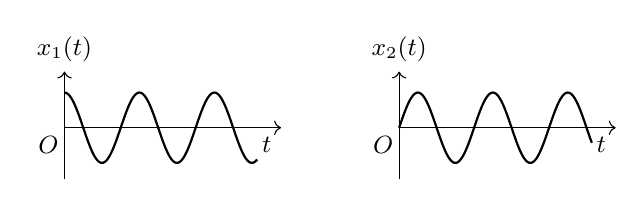
\begin{tikzpicture}[x=1cm,y=0.62cm,every node/.style={font=\small}]
    % ---------- x1(t)=cos(500 pi t) ----------
    \begin{scope}
      \draw[->] (0,0) -- (2.75,0);
      \node[below left] at (2.75,0) {$t$};
      \draw[->] (0,-1.05) -- (0,1.15);
      \node[above] at (0,1.15) {$x_1(t)$};
      \node[below left] at (0.05,0.02) {$O$};
      \draw[thick] plot[samples=240,domain=0:2.45] (\x,{0.72*cos(deg(6.6*\x))});
    \end{scope}
    % ---------- x2(t)=sin(500 pi t) ----------
    \begin{scope}[shift={(4.25,0)}]
      \draw[->] (0,0) -- (2.75,0);
      \node[below left] at (2.75,0) {$t$};
      \draw[->] (0,-1.05) -- (0,1.15);
      \node[above] at (0,1.15) {$x_2(t)$};
      \node[below left] at (0.05,0.02) {$O$};
      \draw[thick] plot[samples=240,domain=0:2.45] (\x,{0.72*sin(deg(6.6*\x))});
    \end{scope}
  \end{tikzpicture}

  \smallskip
  \captionof{figure}{两种可能波形\nobreak：$x_1(t)$ 或 $x_2(t)$}\label{fig:2.2}
\end{center}

% 本灰底框（例2.1 + 例2.2）跨页延续到书 p.38 顶部，框尾文字写在下面。
这样一个随机信号也可以记为\nobreak：$X(t,\xi)=\cos(500\pi t-I(\xi)\pi/2)$\nobreak。其中\nobreak，$I(\xi)$ 是取值 0\nobreak、1 的等概随机变量\nobreak。
\end{examplebox}

在概率论中\nobreak，随机变量 $X$ 是定义在样本空间 $\Omega$ 上的单值实函数\nobreak：它是一种对每个样本点 $\xi$ 赋予一个实数值 $X(\xi)$ 的规则\nobreak。扩展这一概念可建立下面的定义\nobreak，并将它形象地表示为图~\ref{fig:2.3}\nobreak。

\begin{center}
  \begin{tikzpicture}[x=1cm,y=1cm,every node/.style={font=\small}]
    % ---------- 左：样本空间 ----------
    \draw[thick] (0.90,0.20) ellipse (0.72 and 0.58);
    \fill (1.16,0.42) circle (1.3pt);
    \node at (1.33,0.60) {$\xi$};
    \node at (0.90,-0.62) {样本空间 $\Omega$};
    % ---------- 虚线箭头：样本点 $\xi$ 映射为一条时间函数 ----------
    \draw[-{Latex[length=2.2mm]},dashed] (1.58,0.38) .. controls (2.02,0.72) and (2.18,0.30) .. (2.58,0.44);
    % ---------- 右：时间函数空间 ----------
    % 原书框内只有【两条】样本函数，其后接竖排省略号；每条都印有 O 原点与 t 轴标。
    \draw (2.90,-1.72) rectangle (6.20,1.40);
    \begin{scope}[shift={(3.08,0)}]
      % 第一条样本函数
      \draw[->] (0,0.86) -- (2.85,0.86);
      \node[below left] at (2.85,0.86) {$t$};
      \draw[->] (0,0.86) -- (0,1.26);
      \node[left] at (-0.02,0.80) {$O$};
      \draw[thick] plot[samples=220,domain=0:2.55] (\x,{0.86+0.20*sin(deg(30*\x))*(0.65+0.35*sin(deg(1.3*\x)))});
      % 第二条样本函数
      \draw[->] (0,-0.02) -- (2.85,-0.02);
      \node[below left] at (2.85,-0.02) {$t$};
      \draw[->] (0,-0.02) -- (0,0.38);
      \node[left] at (-0.02,-0.08) {$O$};
      \draw[thick] plot[samples=220,domain=0:2.55] (\x,{-0.02+0.18*sin(deg(38*\x+1.0))*(0.65+0.35*sin(deg(1.1*\x+2.0)))});
    \end{scope}
    % 省略号在最后一条样本函数之后（原书位于框底部中央偏右）
    \node at (4.62,-1.18) {$\vdots$};
    \node at (3.30,-1.46) {$X(t,\xi)$};
    \node at (4.55,-2.06) {时间函数空间};
  \end{tikzpicture}

  \smallskip
  \captionof{figure}{定义实函数 $X(t,\xi)$}\label{fig:2.3}
\end{center}

\thm{定义 2.1} 对于随机试验样本空间 $\Omega$ 上每个 $\xi$\nobreak，我们赋予一个函数 $X(t,\xi)$\nobreak，$\xi\in\Omega$\nobreak，则确定了一个具有一定统计特性的随机函数\nobreak，称为随机过程（Stochastic Process or Random Process\nobreak）\nobreak，或随机信号（Random Signal\nobreak）\nobreak。

随机过程是数学上主要使用的术语\nobreak。在工程应用中\nobreak，尤其是在讨论信号与系统的场合\nobreak，我们也常称随机过程为随机信号\nobreak，本书中我们不加区分地使用这两种术语\nobreak。为了便于理解\nobreak，本书中一般采用大写字母表示随机变量与信号\nobreak，小写字母表示确定量与函数\nobreak。

随机信号也可以是离散的\nobreak，如下例所述\nobreak。

\begin{examplebox}
\textbf{例2.3}\quad 医院登记新生儿性别\nobreak。男婴记为 1\nobreak，女婴记为 0\nobreak。这份记录可能是\nobreak：10011010$\cdots$\nobreak，也可能是\nobreak：001010110$\cdots$\nobreak，等等\nobreak。可见这份记录本质上是无穷多种数列中的某个不能事先确知的数列\nobreak，它是具有某种统计规律的随机数列\nobreak。

“新生儿性别记录”问题也可以这样来阐述\nobreak：如果记录中将第 $n$ 个婴儿的性别记为 $X_n(\xi)$\nobreak，那么该记录是序列 $\{X_n(\xi),n=1,2,\cdots\}$\nobreak，参数 $n$ 是正整数\nobreak，每一个 $n$ 对应的 $X_n(\xi)$ 是二值随机变量\nobreak。于是\nobreak，新生儿记录是一列有序的随机变量\nobreak。这份记录事前是完全无法预知的\nobreak，而最终呈现为某种具体的记录结果\nobreak，如图~\ref{fig:2.4} 所示\nobreak。

\begin{center}
  \begin{tikzpicture}[every node/.style={font=\small}]
    \node[circle,draw,minimum size=9.2mm,inner sep=1pt,font=\scriptsize] (c1) at (0,0) {0或1};
    \node[circle,draw,minimum size=9.2mm,inner sep=1pt,font=\scriptsize] (c2) at (1.20,0) {0或1};
    \node[circle,draw,minimum size=9.2mm,inner sep=1pt,font=\scriptsize] (c3) at (2.40,0) {0或1};
    \node at (3.05,0.04) {$\cdots$};
    \draw[-{Latex[length=2.2mm]}] (3.40,0) -- (4.75,0);
    \node at (5.85,0) {01100111$\cdots$};
    \node[below=0.6mm] at (c1.south) {$X_1(\xi)$};
    \node[below=0.6mm] at (c2.south) {$X_2(\xi)$};
    \node[below=0.6mm] at (c3.south) {$X_3(\xi)$};
  \end{tikzpicture}

  \smallskip
  \captionof{figure}{随机变量序列与样本序列}\label{fig:2.4}
\end{center}
\end{examplebox}

上例中的后一种阐述将随机信号看做是含有参量 $n$ 的无穷多个随机变量的集合\nobreak。采用这种方法可以有效地理解例2.1 与例2.2\nobreak，以及其他类似的随机问题\nobreak。

从上面的例子与讨论可以发现\nobreak，随机过程（或信号\nobreak）本质上是一个特殊的二元函数 $X(t,\xi)$\nobreak，其中 $t$ 与 $\xi$ 是具有不同特性的两个自变量\nobreak。$\xi$ 在集合 $\Omega$ 上取值\nobreak，而 $t$ 通常在实数域上取值\nobreak。$\xi$ 的存在表明它具有随机特性\nobreak。应该注意\nobreak，$X(t,\xi)$ 包含了下面几个方面的含义\nobreak：

\begin{citemize}
\item ① 当 $\xi$ 固定时\nobreak，它是 $t$ 的确定函数\nobreak，称此函数为样本函数（Sample Function\nobreak）\nobreak，对应于某次试验的结果\nobreak；
\item ② 当 $t$ 固定时\nobreak，它是一个随机变量\nobreak，说明过程在任何时刻上的取值是不确定的\nobreak。
\item ③ 当 $t$ 与 $\xi$ 都固定时\nobreak，它是一个确定数值\nobreak，称为状态（State\nobreak）\nobreak，如 $X(t)=x$ 就称为“在 $t$ 时刻过程 $X$（的某个试验结果\nobreak）位于 $x$ 状态”\nobreak。
\item ④ 当 $X(t,\xi)$ 的 $t$ 与 $\xi$ 都发生变化时\nobreak，就构成了随机过程（或信号\nobreak）的完整概念\nobreak。
\end{citemize}

这些含义可形象地表示在表 2.1 中\nobreak。

\begin{table}[!ht]
  \centering
  \caption{随机信号 $X(t,\xi)$的含义}\label{tab:2.1}
  \small
  \setlength{\tabcolsep}{4pt}
  \begin{tabular}{c|c|cc}
    \hline
    \shortstack{结果\\ $\xi$} & \shortstack{概率\\ $P[\xi]$} &
    \multicolumn{1}{c|}{\shortstack{随机函数集合\\ $X(t,\xi_i)$}} &
    \shortstack{随机变量集合\\ $X(t_i,\xi)$}\\
    \hline
    $\xi_1$ & $P_1$ &
    \multirow{4}{*}{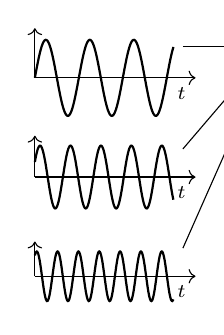
\begin{tikzpicture}[x=0.80cm,y=1.05cm,every node/.style={font=\scriptsize}]
      % 第一条样本函数
      \draw[->] (0,0) -- (2.55,0);
      \draw[->] (0,0) -- (0,0.60);
      \draw[thick] plot[samples=170,domain=0:2.20] (\x,{0.46*sin(deg(9*\x))});
      \node[below left] at (2.55,0) {$t$};
      % 第二条样本函数
      \begin{scope}[shift={(0,-1.20)}]
        \draw[->] (0,0) -- (2.55,0);
        \draw[->] (0,0) -- (0,0.50);
        \draw[thick] plot[samples=200,domain=0:2.20] (\x,{0.38*sin(deg(13*\x+0.5))});
        \node[below left] at (2.55,0) {$t$};
      \end{scope}
      % 第三条样本函数
      \begin{scope}[shift={(0,-2.40)}]
        \draw[->] (0,0) -- (2.55,0);
        \draw[->] (0,0) -- (0,0.42);
        \draw[thick] plot[samples=240,domain=0:2.20] (\x,{0.30*sin(deg(19*\x+1.0))});
        \node[below left] at (2.55,0) {$t$};
      \end{scope}
      % 三条样本函数指向"随机变量集合"的箭头（跨列，overlay 不撑大盒子）
      \draw[overlay,->] (2.35,0.38) -- (3.36,0.38);
      \draw[overlay,->] (2.35,-0.86) -- (3.36,0.04);
      \draw[overlay,->] (2.35,-2.06) -- (3.36,-0.32);
    \end{tikzpicture}} &
    \multirow{4}{*}{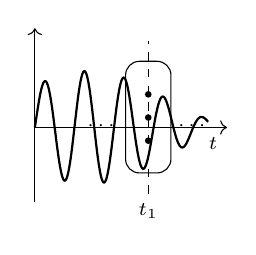
\begin{tikzpicture}[x=0.80cm,y=1.05cm,every node/.style={font=\scriptsize}]
      \draw[->] (0,0) -- (3.05,0);
      \draw[->] (0,-0.90) -- (0,1.20);
      \draw[thick] plot[samples=360,domain=0:2.75]
        (\x,{0.62*sin(deg(10*\x))*(0.55+0.55*sin(deg(1.25*\x+0.5)))});
      \node[below left] at (3.05,0) {$t$};
      % t = t1 处的随机变量：竖直虚线 + 胶囊，表示该时刻的一组取值
      \draw[dashed] (1.80,-0.80) -- (1.80,1.05);
      \draw[rounded corners=5pt] (1.44,-0.55) rectangle (2.16,0.80);
      % 胶囊内沿虚线三个实心点：$t=t_1$ 时刻该随机变量的一组取值
      \fill (1.80,0.40) circle (1.2pt);
      \fill (1.80,0.12) circle (1.2pt);
      \fill (1.80,-0.16) circle (1.2pt);
      \node[below] at (1.80,-0.80) {$t_1$};
      \node at (1.08,0.02) {$\cdots$};
      \node at (2.52,0.02) {$\cdots$};
    \end{tikzpicture}}\\[22pt]
    \cline{1-2}
    $\xi_2$ & $P_2$ & & \\[22pt]
    \cline{1-2}
    $\xi_3$ & $P_3$ & & \\[22pt]
    \cline{1-2}
    $\vdots$ & $\vdots$ & & \\[6pt]
    \hline
  \end{tabular}
\end{table}

通过分析可以看出\nobreak，随机过程是一族样本函数的集合\nobreak，也可以看做一组随机变量的集合\nobreak。数学上常常从后一个观点出发\nobreak，对随机过程做如下的定义\nobreak。

\thm{定义 2.2} 给定某个参量集 $T$\nobreak，若对于每个 $t\in T$\nobreak，都有一个随机变量 $X(t,\xi)$ 与之对应\nobreak，就称依赖于参量 $t$ 的随机变量族 $\{X(t,\xi),t\in T\}$ 为随机过程\nobreak。

定义 2.1 与定义 2.2 在概念上相互补充\nobreak，而本质是一样的\nobreak。前一种定义形式常用于实验观测中\nobreak，通过大量的观测得到充分的样本函数\nobreak，进而可总结出信号的统计规律\nobreak；后一种定义形式在数学上更为严谨\nobreak，常用于理论分析\nobreak。由于将随机信号定义为随机变量的集合\nobreak，使得分析随机信号的问题容易转化为分析随机变量的问题\nobreak。

随机过程常常简记为 $X(t)$\nobreak，其样本函数简记为 $x(t)$\nobreak。参数 $t$ 一般表示时间\nobreak，这正是称之为“过程”或“信号”的原因\nobreak。研究最多的是 $T$ 为实数集 $\R=(-\infty,+\infty)$ 或其子集\nobreak，它可以是有穷或无穷的\nobreak，可列或不可列的\nobreak。如果 $T$ 为整数集或其子集\nobreak，它就是随机序列或离散随机信号\nobreak。这时\nobreak，我们又常改用字母 $n$ 表示参数\nobreak，记为 $X(n)$ 或者 $X_n$\nobreak。

\subsection{基本概率特性}
随机信号是含参数 $t$ 的随机变量族\nobreak，虽然它是不确定的\nobreak，但也是有规律的\nobreak。描述随机信
% EQNUMBERS: （本片无编号公式）
% FIGNUMBERS: 2.1, 2.2, 2.3, 2.4
% TABNUMBERS: 2.1
% PAGES: 37-39
% =====================================================================
%  frag_B —— 书 p.40–42（PDF p.54–56）
%  内容：2.1.2 基本概率特性（续）、2.1.3 基本数字特征、
%        2.2 典型信号举例（起）、2.2.1 随机正弦信号（起）
%  本片编号：式(2.1)(2.2)；图2.5、图2.6；例2.4、例2.5（均为无编号公式）
%  接缝（上）：本片第一行接 frag_A 结尾被分页截断的句子后半截
%        （frag_A 末行 = "……描述随机信"）。assemble_all.py 的 TIGHT_SEAMS
%        已把 A→B 用单个换行接成同一段落，此处不要再加 \noindent。
%  接缝（下）：本片最后一行停在 p.42 末"下面讨论 $X(t)$ 的基本特性。"，
%        p.43 起（2.2.1 的均值推导）由 frag_C 接着写。
% =====================================================================
号的特性可以通过描述带 $t$ 的随机变量 $X(t,\xi)$ 来实现\nobreak。% 本行与 frag_A 末行是同一句话（见 assemble_all.py 的 TIGHT_SEAMS\nobreak）\nobreak，不要加 \noindent

\begin{examplebox}
\textbf{例2.4}\quad 分析例2.2 的掷币试验\nobreak：正面（记为 $H$\nobreak）对应 250\,Hz 频率的余弦波 $\cos(500\pi t)$\nobreak，反面（记为 $T$\nobreak）对应 250\,Hz 的正弦波 $\sin(500\pi t)$\nobreak。求\nobreak：

（1\nobreak）$t=1$\,ms 时随机信号的概率密度与均值\nobreak；（2\nobreak）任意 $t$ 时随机信号的概率密度与均值\nobreak。

\textbf{解}\quad （1\nobreak）在 $t=0.001$s 时\nobreak，随机信号取值为 $X(0.001)$\nobreak，它是一个随机变量\nobreak，不妨简记为 $X_1$\nobreak。易知\nobreak，$X_1$ 可能有两种结果\nobreak：$\cos 0.5\pi$ 或 $\sin 0.5\pi$\nobreak，即 0 或 1\nobreak，概率同为 0.5\nobreak。因此
\[
  f_{X_1}(x)=f_{X(0.001)}(x)=0.5\delta(x)+0.5\delta(x-1)
\]
而且\nobreak，其均值为 $\E X_1=\E[X(0.001)]=0.5$\nobreak。

（2\nobreak）$\forall t$\nobreak，随机信号为一个随机变量\nobreak，简记为 $X_t$\nobreak，其取值为\nobreak：$\cos(500\pi t)$ 或 $\sin(500\pi t)$\nobreak，概率同为 0.5\nobreak。因此
\[
  f_{X(t)}(x)=0.5\delta[x-\cos(500\pi t)]+0.5\delta[x-\sin(500\pi t)]
\]
其均值为\hfill $\E X_t=\E[X(t)]=0.5[\cos(500\pi t)+\sin(500\pi t)]$
\end{examplebox}

上例分析了随机信号在各个孤立时刻上的统计特性\nobreak，简单地讲\nobreak，随机信号的描述同随机变量基本一样\nobreak，只不过附加了参量 $t$ 而已\nobreak。下面的例子进一步分析随机信号在两个时刻上的联合统计特性\nobreak。

\begin{examplebox}
\textbf{例2.5}\quad 分析上例的掷币试验\nobreak。求\nobreak：

（1\nobreak）$t_1=0.5$\,ms 与 $t_2=1$\,ms 时随机信号的二维联合概率密度\nobreak；

（2\nobreak）任意 $t_1,t_2$ 时随机信号的二维联合概率密度\nobreak。

\textbf{解}\quad （1\nobreak）分别简记两时刻上的随机变量为 $X_1=X(0.0005)$ 与 $X_2=X(0.001)$\nobreak，依据掷币结果有\nobreak：

$\xi=H$ 时\nobreak，$\{X_1,X_2\}=\{0.707,0\}$\nobreak，概率为 0.5\nobreak。

$\xi=T$ 时\nobreak，$\{X_1,X_2\}=\{0.707,1\}$\nobreak，概率为 0.5\nobreak。

显然\nobreak，$\{X_1,X_2\}$ 是二维离散随机变量\nobreak，因此
\[
  f_{X_1,X_2}(x,y)=0.5\delta(x-0.707,y)+0.5\delta(x-0.707,y-1)
\]
（2\nobreak）同理\nobreak，$\forall t_1,t_2$\nobreak，记 $X_1=X(t_1)$ 与 $X_2=X(t_2)$\nobreak，依据掷币结果有\nobreak：

$\xi=H$ 时\nobreak，$\{X_1,X_2\}=\{\cos(500\pi t_1),\cos(500\pi t_2)\}$\nobreak，概率为 0.5\nobreak。

$\xi=T$ 时\nobreak，$\{X_1,X_2\}=\{\sin(500\pi t_1),\sin(500\pi t_2)\}$\nobreak，概率为 0.5\nobreak。

因此
\[
  \begin{aligned}
    f_{X_1,X_2}(x,y)=\;&0.5\delta(x-\cos(500\pi t_1),y-\cos(500\pi t_2))\\
    &+0.5\delta(x-\sin(500\pi t_1),y-\sin(500\pi t_2))
  \end{aligned}
\]
\end{examplebox}

由于附带有参量 $t$（或 $t_1,t_2$\nobreak）\nobreak，随机信号的统计特性是随时间（或时间组\nobreak）变化的\nobreak。研究随机信号不只是要分析其具体时刻的统计特性\nobreak，更重要的是要分析这些统计特性随时间（或时间组\nobreak）的变化规律\nobreak。为此\nobreak，我们使用下面的定义\nobreak。

一阶（维\nobreak）概率分布函数定义为任意 $t\in T$ 时刻随机变量 $X(t)$ 的分布函数
\[
  F_X(x;t)=F_{X(t)}(x)=P[X(t)\leqslant x]
\]
因此\nobreak，$F_X(x;t)$ 是 $t$ 时刻的随机变量直至 $x$ 处的累积概率值\nobreak。

一阶（维\nobreak）概率密度函数为
\[
  f_X(x;t)=f_{X(t)}(x)=\frac{\dif}{\dif x}F_X(x;t)
\]

它以时间 $t$ 为参数\nobreak，如图~\ref{fig:2.5} 所示\nobreak。

\begin{wrapfigure}{r}{0.42\textwidth}
  \centering
  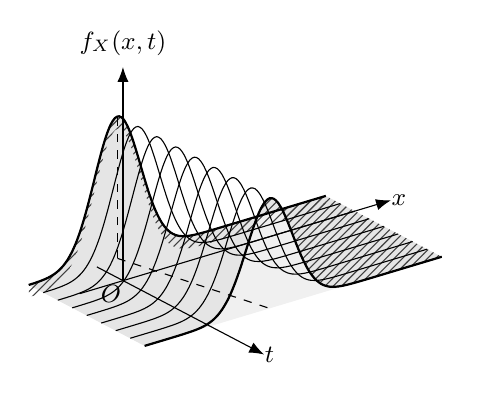
\begin{tikzpicture}[scale=0.92,every node/.style={font=\small},
      declare function={
        hh(\a,\b)=(1.85-0.22*\b)*exp(-((\a-0.45-0.25*\b)/0.45)^2);
        xx(\a,\b)=\a+0.80*\b;
        yy(\a,\b)=0.30*\a-0.42*\b+hh(\a,\b);
        ex0(\a)=\a-0.40;
        ey0(\a)=0.30*\a+0.21+1.96*exp(-((\a-0.325)/0.45)^2);
      }]
    % ---------- 底面：x-t 平面 ----------
    \fill[black!6] (-1.30,-0.06) -- (2.60,1.11) -- (4.20,0.27) -- (0.30,-0.90) -- cycle;
    % ---------- 曲面的"面"：前后缘之间的浅灰面 ----------
    \fill[black!10]
      plot[domain=-0.9:3.2,samples=70,smooth,variable=\a] ({xx(\a,-0.5)},{yy(\a,-0.5)})
      -- plot[domain=3.2:-0.9,samples=70,smooth,variable=\a] ({xx(\a,1.5)},{yy(\a,1.5)})
      -- cycle;
    % ---------- ① 右端的竖直剖面（斜线阴影）----------
    \begin{scope}
      \clip (1.85,-1.20) rectangle (4.60,2.30);
      \fill[pattern=north east lines,pattern color=black!75]
        plot[domain=-0.9:3.2,samples=70,smooth,variable=\a] ({xx(\a,-0.5)},{yy(\a,-0.5)})
        -- plot[domain=3.2:-0.9,samples=70,smooth,variable=\a] ({xx(\a,1.5)},{yy(\a,1.5)})
        -- cycle;
    \end{scope}
    % ---------- ② 曲面下缘沿底面的斜线阴影带 ----------
    \fill[pattern=north east lines,pattern color=black!75]
      plot[domain=-0.9:3.2,samples=70,smooth,variable=\a] ({ex0(\a)},{ey0(\a)})
      -- plot[domain=3.2:-0.9,samples=70,smooth,variable=\a] ({ex0(\a)},{ey0(\a)-0.17})
      -- cycle;
    % ---------- 沿 t 方向的一族 x 截面曲线 ----------
    \foreach \b in {-0.5,-0.25,0,0.25,0.5,0.75,1.0,1.25,1.5}{
      \draw[thin,domain=-0.9:3.2,samples=70,smooth,variable=\a]
        plot ({xx(\a,\b)},{yy(\a,\b)});
    }
    % ---------- 前后缘轮廓 ----------
    \draw[thick,domain=-0.9:3.2,samples=70,smooth,variable=\a]
      plot ({xx(\a,-0.5)},{yy(\a,-0.5)});
    \draw[thick,domain=-0.9:3.2,samples=70,smooth,variable=\a]
      plot ({xx(\a,1.5)},{yy(\a,1.5)});
    % ---------- 坐标轴 ----------
    % 原书如此：图内纵轴标号印成 $f_X(x,t)$（逗号），
    % 与正文一律使用的 $f_X(x;t)$（分号）不一致，照原样保留。
    \draw[-{Latex[length=1.9mm]}] (0,0) -- (0,2.95) node[above=3pt,inner sep=1pt] {$f_X(x,t)$};
    \draw[-{Latex[length=1.9mm]}] (-0.60,-0.18) -- (3.70,1.11) node[right=-1pt,inner sep=1pt] {$x$};
    \draw[-{Latex[length=1.9mm]}] (-0.36,0.19) -- (1.95,-1.02) node[right=-1pt,inner sep=1pt] {$t$};
    \node[below left,inner sep=1pt] at (0.02,-0.02) {$O$};
    % ---------- ③ 底面上沿脊线的虚线投影 ----------
    \draw[dashed,thin] ({xx(0.325,-0.5)},{yy(0.325,-0.5)-hh(0.325,-0.5)})
                    -- ({xx(0.825,1.5)},{yy(0.825,1.5)-hh(0.825,1.5)});
    % ---------- 峰值到 x-t 平面的竖直虚线 ----------
    \draw[dashed] ({xx(0.325,-0.5)},{yy(0.325,-0.5)-hh(0.325,-0.5)})
               -- ({xx(0.325,-0.5)},{yy(0.325,-0.5)});
  \end{tikzpicture}
  \caption{一阶（维\nobreak）密度函数示意图}\label{fig:2.5}
\end{wrapfigure}

二阶（维\nobreak）概率分布函数是 $T$ 上任意两个时刻随机变量 $X(t_1)$ 与 $X(t_2)$ 的联合分布函数
\[
  \begin{aligned}
    F_X(x_1,x_2;t_1,t_2)&=F_{X(t_1)X(t_2)}(x_1,x_2)\\
    &=P[X(t_1)\leqslant x_1,X(t_2)\leqslant x_2]
  \end{aligned}
\]
因此\nobreak，$F_X(x_1,x_2;t_1,t_2)$ 是 $t_1$ 与 $t_2$ 两时刻的随机变量直至 $(x_1,x_2)$ 处的联合累积概率值\nobreak。

二阶（维\nobreak）概率密度函数为
% 原书此式排成一行；本重排版面宽度较原书窄（132mm vs 约 150mm），
% 一行放不下（Overfull 约 17pt），故断成两行，内容不变。
\[
  \begin{aligned}
    f_X(x_1,x_2;t_1,t_2)&=f_{X(t_1)X(t_2)}(x_1,x_2)\\
    &=\frac{\partial^2}{\partial x_1\partial x_2}F_X(x_1,x_2;t_1,t_2)
  \end{aligned}
\]

通过计算边缘分布\nobreak，由二阶分布可以得出一阶分布的结果\nobreak，因此\nobreak，二阶分布比一阶分布包含了更多的信息\nobreak，但也更为复杂\nobreak。

从上述定义中我们注意到\nobreak：随机信号的符号记法与随机变量的相似\nobreak，但习惯地将下标随机变量中的 $t$ 或 $t_1,t_2$ 移到主括号中\nobreak，比如\nobreak，将 $F_{X(t)}(x)$ 改记为 $F_X(x;t)$\nobreak，这样突出了统计特性对于参量的依赖关系\nobreak。后面的讨论中也一直沿用这一习惯\nobreak，我们不再特别提醒\nobreak。此外\nobreak，各种符号中下标 $X$ 表示所针对的随机信号是 $X(t)$\nobreak，在不引起混淆时\nobreak，也可以简化书写\nobreak，省略下标\nobreak。

\subsection{基本数字特征}
例2.4 中我们还分析了信号在各时刻的均值\nobreak，它是一种最基本的数字特征\nobreak。随机信号的数字特征本质上就是带参量的随机变量的数字特征\nobreak，一些基本的数字特征基于单个随机变量 $X(t)$ 或两个变量 $X(t_1)$ 与 $X(t_2)$\nobreak，定义如下\nobreak：

\begin{itemize}
  \setlength{\itemsep}{1pt}
  \item 均值\hfill $m_X(t)=m_{X(t)}=\E[X(t)]$
  \item 方差与标准差\hfill $\sigma_X^2(t)=\sigma_{X(t)}^2=\E[X(t)-m_X(t)]^2$\\
        $\sigma_X^2(t)$ 有时也记为 $\Var[X(t)]$ 或 $D(t)$\nobreak，并且\nobreak，$\sigma_X(t)=\sigma_{X(t)}=\sqrt{\Var[X(t)]}$\nobreak。
  \item 自相关函数\hfill $R_X(t_1,t_2)=\E[X(t_1)X(t_2)]$
  \item 均方值函数\hfill $\E X^2(t)=R_X(t,t)$
  \item 协方差函数\hfill $\begin{aligned}[t]
        C_X(t_1,t_2)&=\Cov(X(t_1),X(t_2))\\
        &=\E\{[X(t_1)-m_X(t_1)][X(t_2)-m_X(t_2)]\}\\
        &=R_X(t_1,t_2)-m_X(t_1)m_X(t_2)
        \end{aligned}$
  \item 相关系数\\[1pt]
        \hfill $\rho_X(t_1,t_2)=\dfrac{\Cov(X(t_1),X(t_2))}{\sigma_{X(t_1)}\sigma_{X(t_2)}}=\dfrac{C_X(t_1,t_2)}{\sigma_X(t_1)\sigma_X(t_2)}$
\end{itemize}

由于定义中的随机变量与参量（时间\nobreak）有关\nobreak，因此\nobreak，随机信号的数字特征都是参量（时间\nobreak）的确定函数\nobreak，反映了物理现象随参量推进的过程感\nobreak。如果分别定义中心化信号与归一化信号为
\begin{equation}
  X_0(t)=X(t)-m_X(t),\qquad \dot{X}(t)=\frac{X(t)-m_X(t)}{\sigma(t)}
  \label{eq:2.1}
\end{equation}

则有
\begin{equation}
  C_X(t_1,t_2)=R_{X_0}(t_1,t_2),\qquad \rho_X(t_1,t_2)=R_{\dot{X}}(t_1,t_2)
  \label{eq:2.2}
\end{equation}

通常\nobreak，$t$ 时刻的均方值反映了随机信号当时的总平均功率\nobreak，均值与标准差反映了其平均特性与摆动范围\nobreak。例如\nobreak，具有正态分布的信号\nobreak，处于区域 $m_X(t)\pm3\sigma(t)$ 的可能性超过 99.74\%\nobreak。% 原书如此\nobreak：正文此处印 $\sigma(t)$\nobreak，而 图2.6 标注为 $\sigma_X(t)$（原书前后不一致\nobreak，照原样保留\nobreak）

\begin{wrapfigure}{r}{0.44\textwidth}
  \centering
  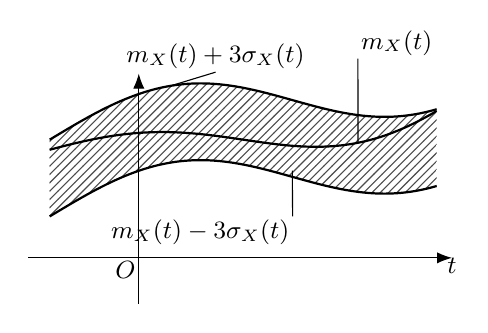
\begin{tikzpicture}[scale=0.78,x=1cm,y=1cm,every node/.style={font=\small}]
    % ---------- 阴影带：下界与上界之间 ----------
    \fill[pattern=north east lines,pattern color=black!70]
      plot[domain=-0.4:5.9,samples=90,smooth,variable=\t]
        ({\t},{2.00+0.55*sin(deg(0.8*\t+0.3))+0.16*\t})
      -- plot[domain=5.9:-0.4,samples=90,smooth,variable=\t]
        ({\t},{2.00+0.55*sin(deg(0.8*\t+0.3))+0.16*\t-1.25})
      -- cycle;
    % ---------- 坐标轴 ----------
    \draw[-{Latex[length=1.9mm]}] (-0.75,0) -- (6.15,0) node[below=-1pt,inner sep=1pt] {$t$};
    \draw[-{Latex[length=1.9mm]}] (1.05,-0.75) -- (1.05,3.00);
    \node[below left,inner sep=1pt] at (1.05,0) {$O$};
    % ---------- 上界 $m_X(t)+3\sigma_X(t)$ ----------
    \draw[thick,domain=-0.4:5.9,samples=90,smooth,variable=\t]
      plot ({\t},{2.00+0.55*sin(deg(0.8*\t+0.3))+0.16*\t});
    % ---------- 下界 $m_X(t)-3\sigma_X(t)$ ----------
    \draw[thick,domain=-0.4:5.9,samples=90,smooth,variable=\t]
      plot ({\t},{2.00+0.55*sin(deg(0.8*\t+0.3))+0.16*\t-1.25});
    % ---------- 中位曲线 $m_X(t)$ ----------
    \draw[thick,domain=-0.4:5.9,samples=90,smooth,variable=\t]
      plot ({\t},{2.00+0.55*sin(deg(0.8*\t+0.3))+0.16*\t-0.30-0.55*sin(deg(0.62*\t))});
    % ---------- 标注与引线 ----------
    % 原书：$m_X(t)+3\sigma_X(t)$ 在左上、$m_X(t)$ 在右上（更高）、$m_X(t)-3\sigma_X(t)$ 在下中，
    % 三者互不重叠，各带一条引线指向对应的曲线（上界 / 中位 / 下界）。
    \node[inner sep=1pt] (up) at (2.30,3.28) {$m_X(t)+3\sigma_X(t)$};
    \draw (up.south) -- (1.60,2.81);
    \node[inner sep=1pt] (mn) at (5.25,3.50) {$m_X(t)$};
    \draw (mn.south west) -- (4.62,1.87);
    \node[inner sep=1pt] (lo) at (2.05,0.42) {$m_X(t)-3\sigma_X(t)$};
    \draw (lo.north east) -- (3.55,1.42);
  \end{tikzpicture}
  \caption{样本函数的最可能出现区域}\label{fig:2.6}
\end{wrapfigure}

利用切比雪夫不等式\nobreak，可以确定一般随机信号样本函数的最可能出现区域\nobreak。这个区域很可能随时间变化\nobreak，如图~\ref{fig:2.6} 所示\nobreak。

虽然上面大量讨论的是连续随机信号的特性与描述方法\nobreak，但对于离散随机信号（或随机序列\nobreak）\nobreak，其结论是类似的\nobreak，只需要将连续时间变量 $t$ 换为离散时间 $n$ 就行了\nobreak。例如\nobreak，一阶分布函数定义为 $F_X(x;n)=P[X(n)\leqslant x]$\nobreak，均值与自相关函数定义为 $m_X(n)=\E[X(n)]$ 与 $R_X(n_1,n_2)=\E[X(n_1)X(n_2)]$\nobreak，等等\nobreak。

\section{典型信号举例}
下面介绍几个简单且极为重要的随机信号\nobreak。我们考虑定义域中的任意时刻 $t$ 与时刻组 $t_1,t_2$\nobreak，讨论信号的均值与相关函数\nobreak，以及一\nobreak、二阶分布与密度函数\nobreak。讨论中示范了常用的分析与计算方法\nobreak。

\subsection{随机正弦信号}
正弦信号是一种在物理与电子工程的科学研究中有着广泛应用的信号\nobreak。随机正弦信号定义为\nobreak：$\{X(t)=A\cos(\Omega t+\Theta),t\in(-\infty,+\infty)\}$\nobreak，其中\nobreak，$A,\Omega$ 与 $\Theta$ 部分或全部是随机变量\nobreak。

电路与系统中\nobreak，几乎总要产生\nobreak、发送与接收正弦信号\nobreak，它本质上都是随机的\nobreak。假定将振荡器设计为产生准确的频率为 5 MHz\nobreak、峰值为 1 V\nobreak、绝对相位为零的正弦信号\nobreak。由于器件与生产工艺固有的容差与不确定性等因素\nobreak，任何的设计与生产者都不可能实际制造出绝对准确的电路与设备\nobreak。设想一下\nobreak，100 件相同的振荡电路\nobreak，同时开启后的结果波形不会是绝对的精确\nobreak，也不会绝对的一模一样\nobreak。再设想一下\nobreak，即便是同一件电路\nobreak，每次开启后也不会呈现出完全一模一样的波形\nobreak。通常幅度与频率可以接近设计值\nobreak，高精度的设备具有较小的差异\nobreak；而初始相位总是难于控制的\nobreak，实际上几乎是完全随机的\nobreak，因此\nobreak，通常近似认为它的数值在整个 $2\pi$ 上均匀分布\nobreak。

再假定用无线方式传输正弦波\nobreak，由于传输过程中受到物理介质内在的不确定性的影响\nobreak，收发两端的距离也无法绝对准确地测量\nobreak，因此\nobreak，收到的信号中\nobreak，幅度经常呈现随机衰落\nobreak，而相位发生未知漂移\nobreak。即使发送的是确定的正弦信号\nobreak，经过传输后它也将是随机的\nobreak。

一种典型的正弦信号是 $X(t)=A\cos(\omega_0t+\Theta)$\nobreak，其中\nobreak，$\omega_0$ 是确定量\nobreak，$A$ 与 $\Theta$ 彼此独立\nobreak，并分别服从参数为 $\sigma^2$ 的瑞利分布与 $[0,2\pi)$ 的均匀分布\nobreak。这种相位服从 $[0,2\pi)$ 均匀分布的信号\nobreak，也统称为随机相位信号（简称随相信号\nobreak）\nobreak。下面讨论 $X(t)$ 的基本特性\nobreak。

% EQNUMBERS: 2.1, 2.2
% FIGNUMBERS: 2.5, 2.6
% PAGES: 40-42

% =====================================================================
%  frag_C —— 书 p.43–45（PDF p.57–59）
%  内容：2.2.1 随机正弦信号（续：均值/自相关/一、二阶密度函数）、
%        2.2.2 伯努利随机序列、2.2.3 半随机二进制传输信号（起）
%  本片编号：式(2.3)–(2.8)，共 6 个；无编号插图、无表格、无例题框
%  接缝（上）：p.43 第一行即 "（1）均值"，是 p.42 起笔的正弦信号分析
%        的继续，本片直接从此行起笔，不重复 p.42 内容。
%  接缝（下）：p.45 最后一行止于 "$\{X_n,n=1,2,\cdots\}$"（句子未完），
%        后半句 "是伯努利序列，$T$ 是某常数值。" 由 frag_D 从 p.46 第一行接着写。
% =====================================================================

（1\nobreak）均值

\begin{equation}
E[X(t)] = E[A]E[\cos(\omega_0 t+\Theta)]
  = E[A]\int_0^{2\pi}\cos(\omega_0 t+\theta)\frac{1}{2\pi}\dif\theta = 0
\label{eq:2.3}
\end{equation}

（2\nobreak）自相关函数

\[
\begin{aligned}
R(t_1,t_2) &= E[A^2]E[\cos(\omega_0 t_1+\Theta)\cos(\omega_0 t_2+\Theta)]\\
&= \frac{1}{2}E[A^2]\bigl\{E[\cos(\omega_0 t_1-\omega_0 t_2)]
   + E[\cos(\omega_0 t_1+\omega_0 t_2+2\Theta)]\bigr\}
\end{aligned}
\]

上式中最后一项均值为 0\nobreak，由于 $A$ 是瑞利分布的\nobreak，于是

\[
\begin{aligned}
E[A^2] &= \int_0^{\infty} r^2\times\frac{r}{\sigma^2}\eu^{-r^2/2\sigma^2}\dif r
  = -\left[r^2\eu^{-r^2/2\sigma^2}\Big|_0^{\infty}
  - \int_0^{\infty}\eu^{-r^2/2\sigma^2}\dif r^2\right]\\
&= -2\sigma^2\eu^{-r^2/2\sigma^2}\Big|_0^{\infty} = 2\sigma^2
\end{aligned}
\]

因而

\begin{equation}
R(t_1,t_2) = \sigma^2\cos\omega_0(t_1-t_2)
\label{eq:2.4}
\end{equation}

式（\ref{eq:2.4}\nobreak）表明\nobreak，信号的相关函数是随时刻间距按正弦规律变化的\nobreak。

（3\nobreak）一\nobreak、二阶密度函数

为了方便书写\nobreak，我们令 $X_1 = X(t_1)$ 与 $X_2 = X(t_2)$\nobreak，其中 $t_1\ne t_2$\nobreak。因此

\[
\begin{cases}
X_1 = g_1(A,\Theta) = A\cos(\omega_0 t_1+\Theta)\\[2pt]
X_2 = g_2(A,\Theta) = A\cos(\omega_0 t_2+\Theta)
\end{cases}
\]

可见\nobreak，$X_1$ 与 $X_2$ 的概率特性能够由 $A$ 与 $\Theta$ 的概率特性得到\nobreak。由于 $A$ 与
$\Theta$ 独立\nobreak，它们的联合密度函数为

\[
f_{A\Theta}(a,\theta) =
\begin{cases}
\dfrac{a}{2\pi\sigma^2}\eu^{-a^2/2\sigma^2}, & a\geqslant 0\\[8pt]
0, & a<0
\end{cases}
\]

计算二元变换的雅克比行列式

\[
\begin{aligned}
J &= \begin{vmatrix}
  \cos(\omega_0 t_1+\theta) & -a\sin(\omega_0 t_1+\theta)\\[2pt]
  \cos(\omega_0 t_2+\theta) & -a\sin(\omega_0 t_2+\theta)
\end{vmatrix}^{-1}\\
&= \frac{1}{a\sin(\omega_0 t_1+\theta)\cos(\omega_0 t_2+\theta)
  - a\cos(\omega_0 t_1+\theta)\sin(\omega_0 t_2+\theta)}\\
&= \frac{1}{a\sin\omega_0(t_1-t_2)}
\end{aligned}
\]

于是\nobreak，利用二元联合密度函数的有关公式得到

\[
f_{X_1X_2}(x_1,x_2) =
\begin{cases}
\dfrac{1}{2\pi\sigma^2\lvert\sin\omega_0(t_1-t_2)\rvert}\eu^{-a^2/2\sigma^2},
  & a\geqslant 0\\[10pt]
0, & a<0
\end{cases}
\]

其中 $a^2$ 应该更换为 $x_1$ 与 $x_2$\nobreak，可如下求得\nobreak：先由

\[
\begin{aligned}
x_1 &= a\cos(\omega_0 t_1+\theta)
     = a\cos\theta\cos\omega_0 t_1 - a\sin\theta\sin\omega_0 t_1\\
x_2 &= a\cos(\omega_0 t_2+\theta)
     = a\cos\theta\cos\omega_0 t_2 - a\sin\theta\sin\omega_0 t_2
\end{aligned}
\]

解出

\[
a\cos\theta = \frac{x_2\sin\omega_0 t_1 - x_1\sin\omega_0 t_2}{\sin\omega_0(t_1-t_2)},
\qquad
a\sin\theta = \frac{x_2\cos\omega_0 t_1 - x_1\cos\omega_0 t_2}{\sin\omega_0(t_1-t_2)}
\]

进而

\[
a^2 = (a\cos\theta)^2 + (a\sin\theta)^2
    = \frac{x_1^2+x_2^2-2x_1x_2\cos\omega_0(t_1-t_2)}{\sin^2\omega_0(t_1-t_2)}
\]

所以

\[
\begin{aligned}
f_{X_1X_2}(x_1,x_2)
&= \frac{1}{2\pi\sigma^2\lvert\sin\omega_0(t_1-t_2)\rvert}
   \exp\left[-\frac{x_1^2+x_2^2-2x_1x_2\cos\omega_0(t_1-t_2)}
   {2\sigma^2\sin^2\omega_0(t_1-t_2)}\right]\\
&= \frac{1}{2\pi\sigma^2\sqrt{1-\rho^2}}
   \exp\left[-\frac{x_1^2+x_2^2-2x_1x_2\rho}{2\sigma^2(1-\rho^2)}\right]
\end{aligned}
\]

其中\nobreak，$\rho = \cos\omega_0(t_1-t_2)$\nobreak。上式其实是 $X_1$ 与 $X_2$ 的二阶概率密度函数\nobreak，
写成规范形式如下

\begin{equation}
\begin{split}
f_X(x_1,x_2;t_1,t_2) &= f_{X_1X_2}(x_1,x_2)
  = \frac{1}{2\pi\sigma^2\lvert\sin\omega_0(t_1-t_2)\rvert}\times\\
&\quad \exp\left[-\frac{x_1^2+x_2^2-2x_1x_2\cos\omega_0(t_1-t_2)}
   {2\sigma^2\sin^2\omega_0(t_1-t_2)}\right]
\end{split}
\label{eq:2.5}
\end{equation}

对照二维正态密度公式可知\nobreak，$X_1,X_2\sim N(0,\sigma^2;0,\sigma^2;\rho)$\nobreak。因此\nobreak，$X_1$ 或
$X_2$ 都服从 $N(0,\sigma^2)$\nobreak。其实 $t_1$ 与 $t_2$ 可以任意\nobreak，它只影响 $\rho$ 的数值\nobreak。
于是\nobreak，该正弦信号的一阶概率密度函数为

\begin{equation}
f_X(x;t) = f_{X_1}(x) = \frac{1}{\sqrt{2\pi}\sigma}\eu^{-x^2/2\sigma^2}
\label{eq:2.6}
\end{equation}

上面两个式子表明\nobreak：信号的一维概率特性不随时间变化\nobreak；二维概率特性随时刻间距变化\nobreak。

从上述分析可看出\nobreak：

\begin{citemize}
\item ① 分析随机信号本质上就是分析相应的随机变量\nobreak；
\item ② 计算均值与相关函数是基本的\nobreak，也是比较容易的\nobreak。而且由它们也容易导出协方差函
数\nobreak、方差等结果\nobreak。例如

\[
C_X(t_1,t_2) = R_X(t_1,t_2) - m_X(t_1)m_X(t_2) = \sigma^2\cos\omega_0(t_1-t_2)
\]

\[
\sigma_X^2(t) = C_X(t,t) = \sigma^2\cos\omega_0(t-t) = \sigma^2
\]

\[
\rho_X(t_1,t_2) = \frac{C_X(t_1,t_2)}{\sigma_X(t_1)\sigma_X(t_2)}
  = \frac{\sigma^2\cos\omega_0(t_1-t_2)}{\sigma^2} = \cos\omega_0(t_1-t_2)
\]

\item ③ 求解密度函数时常常要计算随机变量函数的密度函数\nobreak，可利用概率论中的相应
公式\nobreak。
\end{citemize}

\subsection{伯努利随机序列}
伯努利（Bernoulli\nobreak）序列\nobreak：$\{X_n,n=1,2,\cdots\}$\nobreak，其中各个 $X_n$ 是取值（0,1\nobreak）的
独立\nobreak、同分布二值随机变量\nobreak，即 $X_n\sim B(1,p)$\nobreak，记 $P[X_n=1]=p$\nobreak，$P[X_n=0]=1-p=q$\nobreak。

伯努利序列可以是许多随机现象的数学模型\nobreak，例如\nobreak：

\begin{citemize}
\item ① 在 $n=1,2,3,\cdots$ 时刻独立\nobreak、无休止地进行相同的投币试验\nobreak：1—正面\nobreak；
0—反面\nobreak。
\item ② 给定某个无限长的序列进行试验\nobreak，试验间彼此独立并具有相同分布\nobreak。观测某个事件 B
是否发生\nobreak：1—B 发生\nobreak，0—B 不发生\nobreak。
\item ③ 各种数字通信中\nobreak，串行传输的二进制比特流（常假定各数据位独立\nobreak、同分布\nobreak）\nobreak。伯努
利序列是通信与信息论分析中最常用的数学模型之一\nobreak。
\end{citemize}

伯努利序列的样本序列可以有无穷多种\nobreak，例如\nobreak：

\[
\begin{array}{l}
\{0,\ 1,\ 1,\ 0,\ 1,\ 0,\ \cdots,\ 1,\ 0,\ \cdots\}\\
\{1,\ 1,\ 0,\ 0,\ 0,\ 1,\ \cdots,\ 0,\ 0,\ \cdots\}\\
\{0,\ 1,\ 0,\ 1,\ 0,\ 0,\ \cdots,\ 1,\ 1,\ \cdots\}
\end{array}
\]

下面讨论它的基本特性\nobreak：

（1\nobreak）均值

\begin{equation}
E[X_n] = p\text{\nobreak，即}\quad m(n) = p
\label{eq:2.7}
\end{equation}

（2\nobreak）自相关函数

\[
R(n_1,n_2) = E[X_{n_1}X_{n_2}] =
\begin{cases}
E[X_{n_1}]E[X_{n_2}] = p^2, & n_1\ne n_2\\[6pt]
E[X_{n_1}^2] = p, & n_1 = n_2
\end{cases}
\]

写成紧凑形式有

\begin{equation}
R(n_1,n_2) = pq\delta[n_1-n_2]+p^2
\label{eq:2.8}
\end{equation}

（3\nobreak）一阶概率特性

对于所有 $n$\nobreak，有 $P[X_n=0]=q$\nobreak，$P[X_n=1]=p$\nobreak。如果需要概率密度函数\nobreak，可得到

\[
f(x,n) = f_{X_n}(x) = q\delta(x)+p\delta(x-1)
\]

（4\nobreak）二阶概率特性

观测任意两个时刻 $n_1\ne n_2$\nobreak。令 $P[X_{n_1}X_{n_2}=ab]=P[X_{n_1}=a,X_{n_2}=b]$\nobreak，
对于 $ab$ 的 4 种可能\nobreak：00,01,10,11\nobreak，根据独立性分别有

\[
\begin{array}{@{}l@{\hspace{4em}}l@{}}
P[X_{n_1}X_{n_2}=00]=qq, & P[X_{n_1}X_{n_2}=01]=qp\\[4pt]
P[X_{n_1}X_{n_2}=10]=pq, & P[X_{n_1}X_{n_2}=11]=pp
\end{array}
\]

它是随机序列的“二阶分布律”\nobreak。

至于二阶概率密度函数\nobreak，

\[
f(x_1,x_2;n_1,n_2) = q^2\delta(x_1,x_2) + pq\delta(x_1-1,x_2)
  + pq\delta(x_1,x_2-1) + p^2\delta(x_1-1,x_2-1)
\]

这也可利用独立性\nobreak，由一阶分布求出\nobreak。

% 说明：原书此式第二行排成一行。本重排版心 132mm 排不下（超出 69pt），
%   故在最后一个 "+" 前折行，内容与原书完全相同。
\[
\begin{aligned}
f(x_1,x_2;n_1,n_2) &= [q\delta(x_1)+p\delta(x_1-1)][q\delta(x_2)+p\delta(x_2-1)]\\
&= q^2\delta(x_1)\delta(x_2) + pq\delta(x_1-1)\delta(x_2)
  + pq\delta(x_1)\delta(x_2-1)\\
&\quad + p^2\delta(x_1-1)\delta(x_2-1)
\end{aligned}
\]

注意到\nobreak，$\delta(x_1,x_2)=\delta(x_1)\delta(x_2)$\nobreak，可得到与上面相同的结果\nobreak。

对于 $n_1=n_2$\nobreak，由于 $ab$ 只有两种可能\nobreak：00 与 11\nobreak，而且

\[
\begin{array}{@{}l@{\hspace{4em}}l@{}}
P[X_{n_1}X_{n_2}=00]=q, & P[X_{n_1}X_{n_2}=11]=p
\end{array}
\]

因此\nobreak，由式（1.16\nobreak）得到% 原书如此\nobreak：此处引用的是第 1 章的式(1.16)（离散型密度的冲激表示\nobreak）\nobreak，非笔误

% 原书如此（疑似笔误）：本式第二下标原书印作 n₁，与第一下标相同。
%   24 倍放大、同页同字号并排比对：同页上方那条 f(x₁,x₂;n₁,n₂) 与
%   f(x₁,x₂;n₁,n₂)=[qδ(x₁)+pδ(x₁−1)][qδ(x₂)+pδ(x₂−1)] 的第四下标都是"2"
%   （弯头 + 平底，与同一行的 x₂ 的 2 同形）；而本式第四下标是"1"
%   （竖笔 + 左上小旗 + 小衬线，与本行的 n₁、x₁ 的 1 完全同形）。
%   按保真原则照原样保留 n₁,n₁，不擅自改成 n₂。
\[
f(x_1,x_2;n_1,n_1) = q\delta(x_1,x_2)+p\delta(x_1-1,x_2-1)
\]

伯努利序列是最简单的随机序列\nobreak，其取值是离散的且只有两种可能\nobreak。该序列的均值与一维
概率特性不随时间 $n$ 变化\nobreak；而相关函数与二维概率特性同时刻间距有关\nobreak，分为相同时刻与
不同时刻两种情形\nobreak。

说明\nobreak：分析中要充分利用独立性条件\nobreak。求离散随机变量的密度函数时\nobreak，可先分析取值组合
与有关概率\nobreak，而后再由下面公式直接写出结果\nobreak：

\[
f_X(x) = \sum_i p_i\delta(x-x_i),\qquad
f_{XY}(x,y) = \sum_i\sum_j p_{ij}\delta(x-x_i,y-y_j)
\]

求分布函数时\nobreak，只要将上面公式中的冲激函数改为阶跃函数形式即可\nobreak。

\subsection{半随机二进制传输信号}
半随机二进制传输信号\nobreak：$\{X(t)=2X_n-1,\ (n-1)T\leqslant t<nT,\geqslant 0\}$\nobreak，其中\nobreak，
$\{X_n,n=1,2,\cdots\}$% 本句延续到 p.46 第一行（frag_D 续写“是伯努利序列\nobreak，$T$ 是某常数值\nobreak。”\nobreak）
% 原书如此："(n-1)T ⩽ t < nT, ⩾ 0" 中逗号后直接跟 "⩾ 0"，未见主语；疑原书漏印（或为 n ⩾ 0）
% EQNUMBERS: 2.3, 2.4, 2.5, 2.6, 2.7, 2.8
% FIGNUMBERS: （本片无编号插图）
% TABNUMBERS: （本片无表格）
% PAGES: 43-45
% =====================================================================
%  frag_D —— 书 p.46–48（PDF p.60–62）
%  内容：2.2.3 半随机二进制传输信号（续）、2.2.4 泊松过程
%  本片编号：式(2.9)–(2.17)，图2.7–2.9，表2.2
%  接缝：p.46 第一行"是伯努利序列，$T$ 是某常数值。"是 p.45 下半句的继续
%        （分片 C 结尾停在"…"处）；p.48 最后一行以逗号结束，
%        后半句"号，…"由 frag_E 从 p.49 第一行接着写。
% =====================================================================
是伯努利序列\nobreak，$T$ 是某常数值\nobreak。

在通信中\nobreak，我们称 $T$ 长的时段为 1 个时隙\nobreak，第 $n$ 个时隙是 $t\in[(n-1)T,nT)$\nobreak。因此\nobreak，如果 $\{X_n\}$ 是二进制数据序列\nobreak，那么\nobreak，二进制传输信号描述的是以 $\pm1$ 的电平\nobreak，按 $T$ 宽的时隙\nobreak，逐一承载二进制数据流的传输信号\nobreak。另一种简明的表示形式为
\begin{equation}
\left\{\begin{array}{@{}l@{}}
X(t)=+1,\quad \text{若} X_n=1\\
X(t)=-1,\quad \text{若} X_n=0
\end{array}\right.;
\qquad t\in[(n-1)T,nT)
\label{eq:2.9}
\end{equation}
即 $X(t)=I_n$\nobreak，$t\in[(n-1)T,nT)$\nobreak。其中\nobreak，$\{I_n=2X_n-1,n=1,2,\cdots\}$ 是取值 $(-1,+1)$ 的伯努利序列\nobreak。或者\nobreak，利用方波脉冲信号\nobreak，也可以紧凑地表示为
\[
X(t)=\sum_{n=0}^{\infty}I_{n+1}P_T(t-nT)
\]
式中\nobreak，$P_T(t)$ 是高为 1\nobreak、宽为 $T$ 的方波脉冲\nobreak，它在 $t\in[0,T)$ 时取值为 1\nobreak，其余区域取值为 0\nobreak。如果令 $P_T(t)$ 在 $t\in[-T/2,+T/2)$ 时取值为 1\nobreak，其余区域取值为 0\nobreak，则
% 说明：原书 p.46 上这两个求和式，**第一个（n 从 0 起、$I_{n+1}$）不给编号**，
%       编号 (2.10) 印在**这一个**（n 从 1 起、$I_n$、$t-nT+T/2$）的右侧。
%       （已按 300dpi 扫描页逐像素确认编号的横向位置与哪一行齐平。）
\begin{equation}
X(t)=\sum_{n=1}^{\infty}I_nP_T\left(t-nT+\frac{T}{2}\right)
\label{eq:2.10}
\end{equation}
二进制传输信号的样本函数如图~\ref{fig:2.7}(a)所示\nobreak。

\begin{figure}[htbp]
  \centering
  \begin{tikzpicture}[x=0.70cm,y=0.68cm,every node/.style={font=\small}]
    % ---------- (a) 半随机 ----------
    % 原书波形是 ±1 双极性：低电平压在 −1 刻度上，高电平在 +1；
    % 跳变点在 t=0、T、3T、5T；二进制标注 0 1 1 0 0 1 1 逐时隙对齐。
    \begin{scope}
      \draw[-{Latex[length=2.2mm]}] (0,-1.62) -- (0,1.88);
      \draw[-{Latex[length=2.2mm]}] (-0.50,0) -- (7.75,0);
      \node[above] at (0.05,1.90) {$X(t)$};
      \node[below left] at (7.75,0) {$t$};
      \draw (-0.09,1.00) -- (0.09,1.00);  \node[left] at (-0.14,1.00) {1};
      \draw (-0.09,-1.00) -- (0.09,-1.00); \node[left] at (-0.14,-1.00) {$-1$};
      \node[below left] at (-0.06,-0.06) {0};
      \draw[very thick] (0,-1.00) -- (1,-1.00) -- (1,1.00) -- (3,1.00)
                        -- (3,-1.00) -- (5,-1.00) -- (5,1.00) -- (7.55,1.00);
      \foreach \x/\v in {0.5/0,1.5/1,2.5/1,3.5/0,4.5/0,5.5/1,6.5/1}
        {\node at (\x,1.42) {\v};}
      % 刻度 T / 3T / 5T 标在 t 轴【下方】（原书如此）
      \foreach \x in {1,3,5}{\draw (\x,-0.09) -- (\x,0.09);}
      \node[below] at (1,-0.12) {$T$};
      \node[below] at (3,-0.12) {$3T$};
      \node[below] at (5,-0.12) {$5T$};
      \node at (3.30,-1.98) {\small (a) 半随机};
    \end{scope}
    % ---------- (b) 随机：同一个 ±1 波形整体右移 D ----------
    \begin{scope}[shift={(8.95,0)}]
      \draw[-{Latex[length=2.2mm]}] (0,-1.62) -- (0,1.88);
      \draw[-{Latex[length=2.2mm]}] (-0.50,0) -- (7.75,0);
      \node[above] at (0.05,1.90) {$X(t-D)$};
      \node[below left] at (7.75,0) {$t$};
      \draw (-0.09,1.00) -- (0.09,1.00);  \node[left] at (-0.14,1.00) {1};
      \draw (-0.09,-1.00) -- (0.09,-1.00); \node[left] at (-0.14,-1.00) {$-1$};
      \node[below left] at (-0.06,-0.06) {0};
      % t = D 处的竖直虚线（原书有）
      \draw[dashed] (0.60,-1.45) -- (0.60,1.32);
      % 波形 = (a) 整体右移 D（D = 0.60 < T = 1）
      \draw[very thick] (-0.50,1.00) -- (0.60,1.00) -- (0.60,-1.00) -- (1.60,-1.00)
                        -- (1.60,1.00) -- (3.60,1.00) -- (3.60,-1.00) -- (5.60,-1.00)
                        -- (5.60,1.00) -- (7.55,1.00);
      \foreach \x/\v in {1.10/0,2.10/1,3.10/1,4.10/0,5.10/0,6.10/1,7.10/1}
        {\node at (\x,1.42) {\v};}
      \foreach \x in {1,3,5}{\draw (\x,-0.09) -- (\x,0.09);}
      \node[below] at (1,-0.12) {$T$};
      \node[below] at (3,-0.12) {$3T$};
      \node[below] at (5,-0.12) {$5T$};
      % 随机滑动量 D：双箭头只跨 D（明显小于一个时隙 T），D 写在虚线右侧
      \draw[<->] (0,-1.32) -- (0.60,-1.32);
      \node[right] at (0.66,-1.32) {$D$};
      \node at (3.30,-1.98) {\small (b) 随机};
    \end{scope}
  \end{tikzpicture}
  \caption{半随机与随机二进制传输信号样本函数示例}
  \label{fig:2.7}
\end{figure}

这种信号在通信等领域中大量用到\nobreak，特别是数字通信中\nobreak，它是基带传输信号的基本模型\nobreak，稍微扩展后\nobreak，也是许多其他传输信号的模型\nobreak。上面的几种表现形式都会出现\nobreak，有时还将时间 $t$ 延伸到负无穷\nobreak，即考虑 $t\in(-\infty,+\infty)$\nobreak。我们常称这种信号为半随机的\nobreak，因为其时隙位置准确地与 $t=0$ 对齐\nobreak。在通信应用中\nobreak，这是确知同步时钟的情形\nobreak。更一般的情形中\nobreak，随机二进制传输信号定义为 $Y(t)=X(t-D)$\nobreak，其中 $D$ 与 $X(t)$ 独立\nobreak，是 $[0,T)$ 上均匀分布的随机变量\nobreak。$D$ 引入随机滑动\nobreak，使得时隙边界的位置具有完全的不确定性\nobreak，如图~\ref{fig:2.7}(b)所示\nobreak。下面只讨论半随机二进制传输信号的基本特性\nobreak，随机二进制传输信号将在以后讨论\nobreak。

\bhead{（1\nobreak）均值}
\begin{equation}
m(t)=\E[X(t)]=2\E X_n-1=2p-1=p-q,\qquad t\geqslant 0
\label{eq:2.11}
\end{equation}
\bhead{（2\nobreak）自相关函数}
\[
R(t_1,t_2)=\E[X(t_1)X(t_2)],\qquad t_1\geqslant 0,t_2\geqslant 0
\]
令 $n_1=[\,t_1/T\,]$\nobreak，$n_2=[\,t_2/T\,]$\nobreak，$[\,\ ]$ 是取整运算\nobreak。% 原书此处的取整号是**方括号**（已逐像素 dump 确认\nobreak：左右定界符上下两端各有一条横杠\nobreak，是 [ ] 不是 ⌊ ⌋\nobreak；原书同时用 E[·] 表期望\nobreak，两者同形不冲突\nobreak）\nobreak。以下分两种情况讨论\nobreak。

如果两个时刻位于同一时隙\nobreak，有 $n_1=n_2$\nobreak，则
\[
R(t_1,t_2)=\E[I_n^2]=p+q=1
\]
如果两个时刻位于不同时隙\nobreak，有 $n_1\neq n_2$\nobreak，则
\[
R(t_1,t_2)=\E[I_{n_1}]\E[I_{n_2}]=(2p-1)^2=1-4p(1-p)=1-4pq
\]
合并在一起\nobreak，稍加整理有
\begin{equation}
R(t_1,t_2)=4pq\delta\bigl([\,t_1/T\,]-[\,t_2/T\,]\bigr)+1-4pq,\qquad t_1\geqslant 0,t_2\geqslant 0
\label{eq:2.12}
\end{equation}
多数情况下\nobreak，二进制数据位是等概的\nobreak，即 $p=q=0.5$\nobreak。这时 $m(t)=0$\nobreak，且
\begin{equation}
R(t_1,t_2)=\delta\bigl([\,t_1/T\,]-[\,t_2/T\,]\bigr)=
\begin{cases}
1,& n_1=n_2\\
0,& n_1\neq n_2
\end{cases}
\label{eq:2.13}
\end{equation}
如图~\ref{fig:2.8} 所示\nobreak。

\begin{figure}[htbp]
  \centering
  \scalebox{0.72}{%
  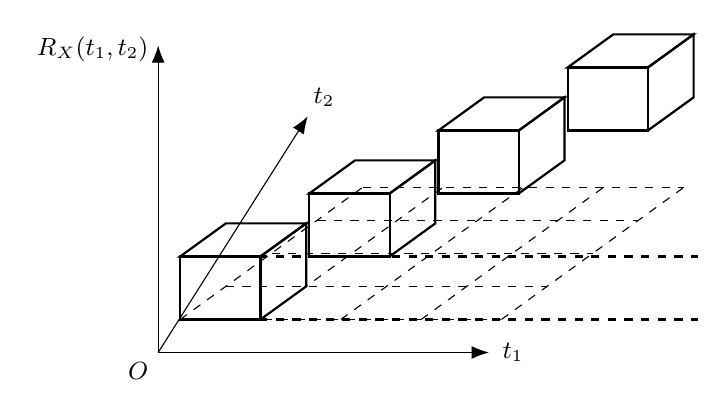
\begin{tikzpicture}[x=1cm,y=1cm,every node/.style={font=\small}]
    % ---------- 坐标轴（等轴测投影）----------
    \draw[-{Latex[length=2.2mm]}] (0,0) -- (4.20,0);
    \node[right] at (4.25,0) {$t_1$};
    \draw[-{Latex[length=2.2mm]}] (0,0) -- (1.90,3.00);
    \node[above right] at (1.85,3.00) {$t_2$};
    \draw[-{Latex[length=2.2mm]}] (0,0) -- (0,3.90);
    \node[left] at (0,3.85) {$R_X(t_1,t_2)$};
    \node[below left] at (0,0) {$O$};
    % ---------- 沿 t1=t2 的取值带：单位立方体串 ----------
    % 屏幕基矢：t1 方向 (1,0)，t2 方向 (0.58,0.75)，R 方向 (0,1)
    \foreach \k in {0,1,2,3}{
      \begin{scope}[shift={({1.02*\k+0.62*\k+0.28},{0.80*\k+0.42})}]
        % 前表面
        \draw[thick] (0,0) -- (1.02,0) -- (1.02,0.80) -- (0,0.80) -- cycle;
        % 右表面
        \draw[thick] (1.02,0) -- (1.60,0.42) -- (1.60,1.22) -- (1.02,0.80);
        % 上表面
        \draw[thick] (0,0.80) -- (1.02,0.80) -- (1.60,1.22) -- (0.58,1.22) -- cycle;
      \end{scope}
    }
    % ---------- 虚等值线（把取值带所在的高度补出来）----------
    \draw[dashed,thick] (0.86,1.22) -- (6.86,1.22);
    \draw[dashed,thick] (0.86,0.42) -- (6.86,0.42);
    % ---------- t1–t2 底面上的虚线网格（原书底面有网格，见 p.47 图2.8）----------
    % 底面基矢：t1 方向 (1.02,0)，t2 方向 (0.58,0.42)，原点在屏幕 (0.28,0.42)
    \foreach \j in {0,1,2,3,4}{%
      \draw[dashed] ({0.28+0.58*\j},{0.42+0.42*\j}) -- ({4.36+0.58*\j},{0.42+0.42*\j});}
    \foreach \i in {0,1,2,3,4}{%
      \draw[dashed] ({0.28+1.02*\i},{0.42}) -- ({0.28+1.02*\i+2.32},{0.42+1.68});}
  \end{tikzpicture}}
  \caption{半随机二进制传输信号的自相关函数示例（$p=q=0.5$\nobreak）}
  \label{fig:2.8}
\end{figure}

\textbf{说明\nobreak：}半随机二进制传输信号可视为伯努利序列的变形\nobreak，它的参量是连续的而取值仍是离散的\nobreak。该信号常表示为式~\eqref{eq:2.9} 与式~\eqref{eq:2.10} 的分段函数形式与方脉冲和的形式\nobreak，适用于不同的计算与分析\nobreak。研究中要处理好参量 $t$ 与 $n$ 的转换\nobreak，使用取整运算是一种有效的方法\nobreak。

\subsection{泊松过程}
泊松（Poisson\nobreak）过程研究的是某种随机现象反复发生的时间点与数目的问题\nobreak，如图~\ref{fig:2.9}所示\nobreak。例如\nobreak：在某个服务窗口前\nobreak，观察一个个顾客前来接受服务的事件\nobreak；又如\nobreak：在某台电话交换机上统计请求通话的事件\nobreak。这些反复发生的随机事件有这样的基本特征\nobreak：① 各个事件“平等”独立\nobreak，且随机发生\nobreak；② 在一定的观察时段上\nobreak，事件的平均发生率稳定\nobreak。

经过适当的数学简化与推导\nobreak，这类随机现象的特性可以更加准确地描述如下\nobreak：

\begin{citemize}
% 原书如此：这里用 $P(\lambda\tau)$ 表示"参数为 $\lambda\tau$ 的泊松分布"（书 p.47 印刷）
\item ① 在任何长度为 $\tau$ 的区间上\nobreak，发生的数目服从泊松分布 $P(\lambda\tau)$\nobreak。其中\nobreak，$\lambda$ 是常数\nobreak，表示单位长度的发生率\nobreak。
\item ② 在不重叠的区间上\nobreak，发生的行为彼此独立\nobreak。
\end{citemize}

泊松过程记为\nobreak：$\{N(t),t\geqslant 0\}$\nobreak，表示直到 $t$ 时刻总的发生数目\nobreak，令其初值为 0\nobreak。可以证明它具有下面的概率特性
\begin{equation}
P[N(t)=k]=\frac{(\lambda t)^k}{k!}\eu^{-\lambda t},\ k=0,1,2,\cdots
\label{eq:2.14}
\end{equation}
它是参数为 $\lambda t$ 的泊松随机变量\nobreak。

许多物理现象发生的时刻与个数是随机的\nobreak，并服从上面描述的规律\nobreak，它们常以泊松过程作为数学模型\nobreak。例如\nobreak：

\begin{citemize}
\item ① 顾客服务\nobreak：在某个服务窗口前\nobreak，观察顾客的总人数\nobreak；
\item ② 故障发生\nobreak：路灯损坏了就立即更换\nobreak，在长期维护中观测更换总个数\nobreak；
\item ③ 电子发射\nobreak：电子枪发射电子流\nobreak，发出电子的总数\nobreak；
\item ④ 误码发生\nobreak：传输数据流时\nobreak，错误码发生总数目\nobreak；
\item ⑤ 电话呼叫\nobreak：某台电话交换机收到呼叫请求的个数\nobreak；
\item ⑥ 网络服务\nobreak：某服务器收到服务请求的个数\nobreak。
\end{citemize}

泊松过程是通信误码分析\nobreak、交换技术与网络业务分析等应用中的一个基本数学模型\nobreak。

\begin{figure}[htbp]
  \centering
  \scalebox{0.92}{%
  \begin{tikzpicture}[x=1cm,y=1cm,every node/.style={font=\small}]
    % ---------- 上：事件发生时刻（泊松点）----------
    \begin{scope}
      \node[anchor=west] at (0,1.62) {事件发生时刻（泊松点\nobreak）\nobreak：};
      \draw[-{Latex[length=2.2mm]}] (0,0.95) -- (12.35,0.95);
      \node[below left] at (12.35,0.95) {$t$};
      \node[below] at (0.02,0.90) {$O$};
      \foreach \x/\lab in {1.55/{$S_1$},3.60/{$S_2$},4.70/{$S_3$},6.45/{},8.55/{$S_k$},10.35/{},11.45/{}}
        {\draw (\x,0.88) -- (\x,1.02);
         \node[below=1pt] at (\x,0.86) {\lab};}
    \end{scope}
    % ---------- 下：泊松计数 N(t) ----------
    \begin{scope}[shift={(0,-3.30)}]
      \draw[-{Latex[length=2.2mm]}] (0,0) -- (0,3.05);
      \draw[-{Latex[length=2.2mm]}] (0,0) -- (12.35,0);
      \node[above] at (0,3.05) {$N(t)$（事件计数\nobreak）};
      \node[below left] at (12.35,0) {$t$};
      \node[below left] at (0,0) {$O$};
      % 阶梯：事件时刻处在 t_i 处跳一级
      \draw[very thick] (0,0) -- (1.55,0) -- (1.55,0.50) -- (3.60,0.50) -- (3.60,1.00)
        -- (4.70,1.00) -- (4.70,1.50) -- (6.45,1.50) -- (6.45,2.00) -- (8.55,2.00)
        -- (8.55,2.50) -- (11.45,2.50) -- (11.45,2.90) -- (12.10,2.90);
      % 事件时刻（轴上的 × 标记）
      \foreach \x in {1.55,3.60,4.70,6.45,8.55,11.45}{\node at (\x,-0.02) {$\times$};}
      % k 与 t_k 的标注
      \draw[dashed] (0,2.50) -- (8.55,2.50);
      \draw[dashed] (8.55,0) -- (8.55,2.50);
      \node[left] at (0,2.50) {$k$};
      \node[below] at (8.55,-0.06) {$t_k$};
      \draw[-{Latex[length=2.2mm]}] (10.95,1.75) -- (11.50,0.22);% 原书箭头指向 t_k 竖虚线【右侧\nobreak】的那个 ×（第 6 个事件点\nobreak）\nobreak，不是 t_k 处的 ×
      \node[anchor=west] at (11.00,1.75) {事件时刻};
    \end{scope}
  \end{tikzpicture}}
  \caption{泊松事件时刻与泊松计数的样本函数示例}
  \label{fig:2.9}
\end{figure}

下面讨论泊松过程的基本特性\nobreak，其中\nobreak，$t\geqslant 0,t_1\geqslant 0,t_2\geqslant 0$\nobreak。

\bhead{（1\nobreak）均值}
根据 1.6 节泊松随机变量的均值与方差等结果\nobreak，容易得到
\begin{equation}
m(t)=\E[N(t)]=\lambda t
\label{eq:2.15}
\end{equation}
\bhead{（2\nobreak）自相关函数}
不妨先考虑 $t_2\geqslant t_1$\nobreak，令 $\tau=t_2-t_1$\nobreak。利用泊松过程的特性（1\nobreak）可知\nobreak，在 $[t_1,t_2)$ 上的发生个数是参数为 $\lambda\tau$ 的泊松随机变量\nobreak，因此就是 $N(\tau)$\nobreak。于是
\begin{align*}
R(t_1,t_2)&=\E[N(t_1)N(t_2)]=\E\{N(t_1)[N(t_1)+N(\tau)]\}\\
&=\E\left[N^2(t_1)\right]+\E[N(t_1)N(\tau)]
\end{align*}
再利用泊松过程的特性（2\nobreak）有
\[
\E[N(t_1)N(\tau)]=\E[N(t_1)]\E[N(\tau)]
\]
又根据泊松随机变量的均值与方差等结果\nobreak，有
\begin{align*}
\E[N(t_1)]&=\lambda t_1\\
\E[N(\tau)]&=\lambda\tau=\lambda(t_2-t_1)\\
\E\left[N^2(t_1)\right]&=D[N(t_1)]+\{\E[N(t_1)]\}^2=\lambda t_1+(\lambda t_1)^2
\end{align*}
所以
\[
R(t_1,t_2)=\lambda t_1+\lambda^2t_1t_2
\]
当 $t_2<t_1$ 时\nobreak，由 $R(t_1,t_2)$ 的对称性\nobreak，将上式中 $t_1$ 与 $t_2$ 互换即可\nobreak。综合起来最后有
\begin{equation}
R(t_1,t_2)=\lambda\min(t_1,t_2)+\lambda^2t_1t_2
\label{eq:2.16}
\end{equation}
\bhead{（3\nobreak）一阶概率特性}
泊松过程 $N(t)\sim P(\lambda t)$\nobreak，由于取值是离散的\nobreak，采用概率形式更简洁\nobreak，即
\[
P[N(t)=k]=\frac{(\lambda t)^k}{k!}\eu^{-\lambda t},\ k=0,1,2,\cdots
\]
也有很多的时候使用其特征函数\nobreak。利用 1.6 节泊松随机变量的相应结果\nobreak，可以得出
\begin{equation}
\phi(v;t)=\E\left[\eu^{\ju vN(t)}\right]=\exp\left[\lambda t\left(\eu^{\ju v}-1\right)\right]
\label{eq:2.17}
\end{equation}
\textbf{说明\nobreak：}分析泊松信号时要充分利用它的两个特性\nobreak，如在上面自相关函数的计算中\nobreak。需要用到泊松变量的有关结果时\nobreak，可在 1.6 节中找到\nobreak。

最后\nobreak，通过上面几个简单例子及其分析\nobreak，我们注意到\nobreak：

\begin{citemize}
\item ① 上面几个简单例子给出了几个重要的随机信号\nobreak，它们是多种实际物理现象的模型\nobreak。
\item ② 上面几个简单例子示范了随机信号的几种基本类型\nobreak，如表 2.2 所示\nobreak。
\end{citemize}

\begin{center}
  \captionof{table}{随机信号的基本类型}\label{tab:2.2}

  \small
  \setlength{\tabcolsep}{6pt}
  \begin{tabular}{|c|c|c|}
    \hline
     & 连续值域 & 离散值域\\
    \hline
    连续参量 & 正弦信号 & （半随机\nobreak）二进制传输信号\nobreak，泊松信号\\
    \hline
    离散参量 & — & 伯努利序列\\
    \hline
  \end{tabular}
\end{center}

\begin{citemize}
\item ③ 一般而言\nobreak，随机信号的统计特性是随参量变化的\nobreak，表现出规律性\nobreak。
\item ④ 简单地讲\nobreak，分析随机信号本质上就是分析相应的随机变量\nobreak。其中\nobreak，计算均值与相关函数是基本的\nobreak，由它们容易导出协方差函数与方差等结果\nobreak。求解概率特性时\nobreak，对于取值连续的信号\nobreak，常常要计算随机变量函数的密度函数\nobreak，可利用有关定理与公式\nobreak；对于取值离散的信
% ★ 本条目④的句子在书 p.48 末被页边界切断，后半截「号，通常应先直接计算有关概率……
%   形式来表示。」印在书 p.49 第一行。这一段话**仍是条目④的一部分**，所以：
%     · 本片**故意不写** \end{citemize}（与 frag_H 故意不写 \end{examplebox} 同例）；
%     · \end{citemize} 写在 frag_E.tex 里、那句话结束之后；
%     · assemble_all.py 的 TIGHT_SEAMS 已把 ("D","E") 列为同段接缝。
%   代价：frag_D 单独试编译时列表不配平，在 harness 的 \input 后补一行 \end{citemize} 即可。
% EQNUMBERS: 2.9, 2.10, 2.11, 2.12, 2.13, 2.14, 2.15, 2.16, 2.17
% FIGNUMBERS: 2.7, 2.8, 2.9
% TABNUMBERS: 2.2
% PAGES: 46-48
% =====================================================================
%  frag_E —— 书 p.49–51（PDF p.63–65）
%  内容：2.3 一般特性与基本运算、2.3.1 n 阶概率特性、2.3.2 联合特性
%        （含 定义2.3、例2.6、例2.7）
%  ★ 本片编号公式数 = 0 ★
%    p.49–52（2.3.1 / 2.3.2 / 2.3.3）原书确实没有任何带编号的公式，
%    已用 3×–8× 放大逐一复核右边距。本片所有独立居中公式一律用 \[ \]，
%    绝不用 equation（否则第2章其后所有编号整体后移，xelatex 不报错）。
%    上一号 (2.17) 在书 p.48（frag_D）；下一号 (2.18) 在书 p.53（frag_F）。
%  接缝：
%    * 本片第一行是 p.48 末句「…对于取值离散的信」的续行 —— frag_D 结尾
%      停在“信”字，本片从“号，通常应先…”接起，不重复 p.48 的内容。
%    * 正文「如 1.4 节所述」「三者的关系仍如图 1.12 所示」是跨章引用，
%      指第1章 §1.4 与 图1.12，原书如此，原样保留（不是笔误，不要改成 图2.x）。
%    * 正文「因此利用式（2.5）有」引用的是 frag_C 里的 (2.5)，原样保留。
%  灰底框：
%    * p.50 末 例2.6 的灰底框跨到 p.51 上部才结束（本片内自行闭合）。
%    * p.51 中下部 例2.7 另起一个新的灰底框，到 p.51 末尾结束。
%  说明：原书这些“标签＋公式”同行排的段落（互相关函数：/ 式中 / 即 /
%        于是）用非浮动 center+tabular 还原其两栏结构。
% =====================================================================
号\nobreak，通常应先直接计算有关概率\nobreak，需要密度（或分布\nobreak）函数时\nobreak，再用其冲激（或阶跃\nobreak）函数形式来表示\nobreak。
\end{citemize}
% ↑ 本行是 frag_D 末尾 ④ 条目那句话的续行（书 p.48 末 → p.49 首，页边界切断）。
%   它是**条目④的一部分**，故 \end{citemize} 由本片补上，frag_D 故意不写（见 frag_D 的接缝注释）。
%   assemble_all.py 的 TIGHT_SEAMS 把 ("D","E") 列为同段接缝，装配后两行之间没有空行。

\section{一般特性与基本运算}
前面我们详细讨论了随机信号 $X(t)$ 的一\nobreak、二阶分布与矩的基本特性\nobreak。由于 $X(t)$ 是无穷多个随机变量的总体\nobreak，因此\nobreak，要全面地描述它的统计特性必须用到其任意有穷阶分布\nobreak。我们下面讨论它的一些更一般的特性\nobreak。

讨论中只考虑连续参数的随机信号 $X(t)$\nobreak。下面的定义与结论\nobreak，除积分与导数运算外\nobreak，同样适用于离散随机信号（或随机序列\nobreak）$X(n)$\nobreak，只需要将连续时间变量 $t$ 换为离散时间变量 $n$ 就行了\nobreak。本章后面各节中也大都如此\nobreak，我们不再特别说明\nobreak。

\subsection{$n$ 阶概率特性}
随机信号 $\{X(t),t\in T\}$ 的 $n$ 阶（维\nobreak）概率特性由它的任意 $n$ 个时刻 $t_1,t_2,\cdots,t_n\in T$ 上的随机变量 $X(t_1),X(t_2),\cdots,X(t_n)$ 来定义\nobreak。它的 $n$ 阶（维\nobreak）概率分布函数定义为
\[
F(x_1,x_2,\cdots,x_n;t_1,t_2,\cdots,t_n)=P[X(t_1)\leqslant x_1, X(t_2)\leqslant x_2,\cdots,X(t_n)\leqslant x_n]
\]
其 $n$ 阶（维\nobreak）概率密度函数定义为 $f(x_1,x_2,\cdots,x_n;t_1,t_2,\cdots,t_n)$\nobreak，它满足
\[
\resizebox{\linewidth}{!}{$\displaystyle
F(x_1,x_2,\cdots,x_n;t_1,t_2,\cdots,t_n)
=\int_{-\infty}^{x_n}\cdots\int_{-\infty}^{x_2}\int_{-\infty}^{x_1}
f(x_1,x_2,\cdots,x_n;t_1,t_2,\cdots,t_n)\dif x_1\dif x_2\cdots\dif x_n$}
\]
对于连续型信号有
\[
f(x_1,x_2,\cdots,x_n;t_1,t_2,\cdots,t_n)
=\frac{\partial^n}{\partial x_1\partial x_2\cdots\partial x_n}
F(x_1,x_2,\cdots,x_n;t_1,t_2,\cdots,t_n)
\]

还可以定义它的 $n$ 维特征函数为
\[
\phi(v_1,v_2,\cdots,v_n;t_1,t_2,\cdots,t_n)
=E\left\{\exp\left[\ju\left(v_1X(t_1)+v_2X(t_2)+\cdots+v_nX(t_n)\right)\right]\right\}
\]

2.1 节讨论随机信号 $X(t)$ 的一\nobreak、二阶分布时\nobreak，我们注意到二阶分布比一阶分布包含了更多的信息\nobreak。可以想象\nobreak，如果时刻点取得越多\nobreak，用到的高阶分布的阶数越高\nobreak，则对信号特性的描述也越趋完善\nobreak。理论上讲\nobreak，无限地增加时刻点数\nobreak，缩小时刻间距\nobreak，可以全面地反映出信号的统计特性\nobreak。
一般而言\nobreak，求取高阶分布是不容易的\nobreak，除非随机信号在不同时刻的随机变量是彼此独立的\nobreak。例如\nobreak，伯努利序列的 $n$ 阶密度函数是其一阶密度函数的乘积\nobreak，即
\[
f(x_1,x_2,\cdots,x_n;t_1,t_2,\cdots,t_n)
=\prod_{i=1}^{n}f(x_i;t_i)
=\prod_{i=1}^{n}\left[q\delta(x_i)+p\delta(x_i-1)\right]
\]

实际应用时往往不必（也可能无法\nobreak）获得较高阶的分布特性\nobreak，而只需要一\nobreak、二阶分布就可以解决大量问题\nobreak，甚至仅需要几个基本的数字特征即可\nobreak。

\subsection{联合特性}
研究多个随机信号及相互关系时\nobreak，要用到联合特性\nobreak。两个信号 $X(t)$ 与 $Y(t)$ 的联合概率分布函数由它们任意两个时刻的随机变量 $X(t_1)$ 与 $Y(t_2)$ 来定义\nobreak，即
\[
F_{XY}(x,y;t_1,t_2)=F_{X(t_1)Y(t_2)}(x,y)=P[X(t_1)\leqslant x, Y(t_2)\leqslant y]
\]
进而\nobreak，它们的 $(n+m)$ 维联合概率分布函数定义为
\[
\resizebox{\linewidth}{!}{$\displaystyle
\begin{aligned}
&F_{XY}(x_1,x_2,\cdots,x_n;y_1,y_2,\cdots,y_m;t_1,t_2,\cdots,t_n;s_1,s_2,\cdots,s_m)\\
&=P[X(t_1)\leqslant x_1, X(t_2)\leqslant x_2,\cdots,X(t_n)\leqslant x_n; Y(s_1)\leqslant y_1, Y(s_2)\leqslant y_2,\cdots,Y(s_m)\leqslant y_m]
\end{aligned}$}
\]

相仿地可定义 $X(t)$ 与 $Y(t)$ 的联合概率密度函数与特征函数\nobreak。

信号 $X(t)$ 与 $Y(t)$ 的基本联合数字特征是互相关函数\nobreak、互协方差函数与互相关系数\nobreak。它们基于随机变量 $X(t_1)$ 与 $Y(t_2)$ 的定义如下\nobreak：

\begin{center}
\begin{tabular}{@{}l@{\hspace{1.5em}}l@{}}
\textbf{互相关函数\nobreak：} & $\displaystyle R_{XY}(t_1,t_2)=E[X(t_1)Y(t_2)]$\\[4pt]
\textbf{互协方差函数\nobreak：} & $\displaystyle
\begin{aligned}
C_{XY}(t_1,t_2)&=\Cov(X(t_1),Y(t_2))\\
&=E\{[X(t_1)-m_X(t_1)][Y(t_2)-m_Y(t_2)]\}\\
&=R_{XY}(t_1,t_2)-m_X(t_1)m_Y(t_2)
\end{aligned}$\\[4pt]
\textbf{互相关系数\nobreak：} & $\displaystyle \rho_{XY}(t_1,t_2)=\frac{C_{XY}(t_1,t_2)}{\sigma_X(t_1)\sigma_Y(t_2)}$
\end{tabular}
\end{center}

由上可见\nobreak，$R_{XX}(t_1,t_2)$ 也就是 $R_X(t_1,t_2)$\nobreak，有的文献中常采用这种记法\nobreak。% 原书如此\nobreak：此处印作 R_{XX}（前文定义的是 R_{XY}\nobreak）\nobreak，已 7× 放大确认
关于两个随机信号的关系\nobreak，我们有下面的定义\nobreak。

\thm{定义 2.3} 若对于所有 $t_1,t_2\in T$ 恒有
\begin{citemize}
\item ① $R_{XY}(t_1,t_2)=0$\nobreak，则称信号 $\{X(t),t\in T\}$ 与 $\{Y(t),t\in T\}$ 彼此正交\nobreak。
\item ② $C_{XY}(t_1,t_2)=0$\nobreak，即 $E[X(t_1)Y(t_2)]=E[X(t_1)]E[Y(t_2)]$\nobreak，则称信号 $\{X(t),t\in T\}$ 与 $\{Y(t),t\in T\}$ 彼此无关\nobreak。
\end{citemize}

相仿地\nobreak，若从两个信号中取得的任意随机变量组彼此独立\nobreak，则称信号 $\{X(t),t\in T\}$ 与 $\{Y(t),t\in T\}$ 彼此独立\nobreak。其充要条件是\nobreak：任取 $t_1,t_2,\allowbreak\cdots,t_n,\allowbreak s_1,s_2,\allowbreak\cdots,s_m\in T$\nobreak，恒有
\[
\begin{aligned}
&F_{XY}(x_1,x_2,\cdots,x_n;y_1,y_2,\cdots,y_m;t_1,t_2,\cdots,t_n;s_1,s_2,\cdots,s_m)\\
&=F_X(x_1,x_2,\cdots,x_n;t_1,t_2,\cdots,t_n)F_Y(y_1,y_2,\cdots,y_m;s_1,s_2,\cdots,s_m)
\end{aligned}
\]
显然\nobreak，该条件也可用相应的密度函数或特征函数进行表述\nobreak，其形式是相似的\nobreak。

如 1.4 节所述\nobreak，正交与无关是基于二阶矩的概念\nobreak，而独立性是基于概率特性的概念\nobreak，独立性的概念更为苛刻\nobreak，三者的关系仍如图 1.12 所示\nobreak。

$n$ 个随机信号集中在一起构成 $n$ 维向量随机信号\nobreak，形如 $(X_1(t),X_2(t),\allowbreak\cdots,\allowbreak X_n(t))$\nobreak。它的概率特性由这 $n$ 个随机信号各自的\nobreak，以及联合的统计特性所规定\nobreak。例如\nobreak，二维随机游动点的平面坐标 $\{(X(t),Y(t)),t\in T\}$\nobreak，本质上是两个关联的随机信号\nobreak。另一方面\nobreak，如果参数的取值是多维的\nobreak，则称其为多参量随机信号\nobreak，或随机场\nobreak。例如\nobreak，某时刻全国各地的温度值\nobreak，$\{T(x,y),x,y\in\R^2\}$\nobreak，参量是地域坐标\nobreak；或者一幅数字图像 $\{V(x,y),1\leqslant x,y\leqslant 1024\}$\nobreak。这些形式的随机信号的分析建立在基本随机信号的基础上\nobreak，本书不做深入讨论\nobreak。
% 上句原书印作斜体 $R^2$；本处按全书统一用宏 \R（实数集），参见 frag_A 的 $\R=(-\infty,+\infty)$。

% 本灰底框（例2.6）自 p.50 末尾起，延续到 p.51 上部才结束。
\begin{examplebox}
\textbf{例2.6}\quad 讨论随机信号 $Z(t)=aX(t)+bY(t)$ 的均值\nobreak、相关函数与协方差函数\nobreak，其中 $a$ 与 $b$ 是确定量\nobreak。

\textbf{解}\nobreak：根据定义有
\[
E[Z(t)]=aE[X(t)]+bE[Y(t)]=am_X(t)+bm_Y(t)
\]
\[
\begin{aligned}
R_Z(t_1,t_2)&=E\{[aX(t_1)+bY(t_1)][aX(t_2)+bY(t_2)]\}\\
&=a^2R_X(t_1,t_2)+b^2R_Y(t_1,t_2)+abR_{XY}(t_1,t_2)+baR_{YX}(t_1,t_2)
\end{aligned}
\]
其中涉及到两个信号的互相关函数\nobreak。如果 $X(t)$ 与 $Y(t)$ 正交\nobreak，则
\[
R_Z(t_1,t_2)=a^2R_X(t_1,t_2)+b^2R_Y(t_1,t_2)
\]

考虑减去均值的中心化信号 $Z_0(t)=aX_0(t)+bY_0(t)$\nobreak，于是
\[
R_{Z_0}(t_1,t_2)=a^2R_{X_0}(t_1,t_2)+b^2R_{Y_0}(t_1,t_2)+abR_{X_0Y_0}(t_1,t_2)+baR_{Y_0X_0}(t_1,t_2)
\]
\begin{center}
\begin{tabular}{@{}l@{\hspace{0.9em}}l@{}}
即 & $\displaystyle C_Z(t_1,t_2)=a^2C_X(t_1,t_2)+b^2C_Y(t_1,t_2)+abC_{XY}(t_1,t_2)+baC_{YX}(t_1,t_2)$
\end{tabular}
\end{center}
其中涉及到两个信号的互协方差函数\nobreak。如果 $X(t)$ 与 $Y(t)$ 无关\nobreak，则
\[
C_Z(t_1,t_2)=a^2C_X(t_1,t_2)+b^2C_Y(t_1,t_2)
\]
\end{examplebox}

% 例2.7 的灰底框：p.51 中下部起，到 p.51 末结束。
\begin{examplebox}
\textbf{例2.7}\quad 讨论两个信号 $R(t)=A\cos(\omega_0t+\Theta)$ 与 $I(t)=A\sin(\omega_0t+\Theta)$\nobreak。其中 $A$ 与 $\Theta$ 为实随机变量\nobreak，且彼此独立\nobreak。假定 $A$ 服从参数为 $\sigma^2$ 的瑞利分布\nobreak，$\Theta$ 在 $[-\pi,\pi]$ 上均匀分布\nobreak。

（1\nobreak）讨论它们的联合概率特性\nobreak；（2\nobreak）讨论它们的互相关函数及正交与无关性\nobreak。

\textbf{解}\nobreak：（1\nobreak）$R(t)$ 与 $I(t)$ 为随机正弦信号\nobreak，它们最基本的联合密度函数是 $R(t_1)$ 与 $I(t_2)$ 之间的联合密度函数\nobreak，可仿照 2.2 节中的方法求出\nobreak，先建立 $R(t_1)$\nobreak、$I(t_2)$ 与 $A$\nobreak、$\Theta$ 的函数关系\nobreak，然后有
\[
f_{RI}(r,i;t_1,t_2)=f_{A\Theta}(a,\theta)\lvert J\rvert
\]
\begin{center}
\begin{tabular}{@{}l@{\hspace{1.5em}}l@{}}
式中 & $\displaystyle J=\begin{vmatrix}
\cos(\omega_0t_1+\theta) & -a\sin(\omega_0t_1+\theta)\\
\sin(\omega_0t_2+\theta) & a\cos(\omega_0t_2+\theta)
\end{vmatrix}^{-1}=\frac{1}{a\cos\omega_0(t_1-t_2)}$
\end{tabular}
\end{center}

另一种方法是借助已有的结果\nobreak，注意到 $R(t)$ 与 2.2 节中分析的随机正弦信号相同\nobreak，而
\[
I(t)=A\sin(\omega_0t+\Theta)
=A\cos\left[\omega_0\left(t-\frac{\pi}{2\omega_0}\right)+\Theta\right]
=R\left(t-\frac{\pi}{2\omega_0}\right)
\]
因此利用式（2.5\nobreak）有
\[
\begin{aligned}
f_{RI}(r,i;t_1,t_2)&=f_{RR}\left(r,i;t_1,t_2-\frac{\pi}{2\omega_0}\right)\\
&=\frac{1}{2\pi\sigma^2\lvert\cos\omega_0(t_1-t_2)\rvert}
\exp\left[-\frac{r^2+i^2+2ri\sin\omega_0(t_1-t_2)}{2\sigma^2\cos^2\omega_0(t_1-t_2)}\right]\\
&=\frac{1}{2\pi\sigma^2\sqrt{1-\rho^2}}
\exp\left[-\frac{r^2+i^2-2ri\rho}{2\sigma^2(1-\rho^2)}\right]
\end{aligned}
\]
这里\nobreak，$\rho=-\sin\omega_0(t_1-t_2)$\nobreak，它显然也是正态分布的\nobreak。

对于 $(1+1)$ 阶以上的联合概率特性\nobreak，这里不再分析\nobreak。

（2\nobreak）$R(t)$ 与 $I(t)$ 都是随机正弦信号\nobreak，易知\nobreak，$E[R(t)]=E[I(t)]=0$\nobreak。再分析 $R(t)$ 与 $I(t)$ 之间的互相关性
\[
R_{RI}(t_1,t_2)=E[A^2\cos(\omega_0t_1+\Theta)\sin(\omega_0t_2+\Theta)]=\frac{1}{2}E[A^2]\sin\omega_0(t_2-t_1)
\]
\[
R_{IR}(t_1,t_2)=E[A^2\sin(\omega_0t_1+\Theta)\cos(\omega_0t_2+\Theta)]=\frac{1}{2}E[A^2]\sin\omega_0(t_1-t_2)
\]
\begin{center}
\begin{tabular}{@{}l@{\hspace{1.5em}}l@{}}
于是 & $\displaystyle C_{RI}(t_1,t_2)=R_{RI}(t_1,t_2)=\frac{1}{2}E[A^2]\sin\omega_0(t_2-t_1)$\\[4pt]
 & $\displaystyle C_{IR}(t_1,t_2)=R_{IR}(t_1,t_2)=\frac{1}{2}E[A^2]\sin\omega_0(t_1-t_2)$
\end{tabular}
\end{center}

可见\nobreak，两个信号间的互相关函数值是随时间刻间距而变的\nobreak。$R_{RI}(t,t)=C_{RI}(t,t)=0$\nobreak，表明在同一时刻\nobreak，两信号上的随机变量 $R(t)$ 与 $I(t)$ 正交且无关\nobreak。但整个信号 $\{R(t),t\in(-\infty,+\infty)\}$ 与 $\{I(t),t\in(-\infty,+\infty)\}$ 之间非正交\nobreak，也相关\nobreak。
\end{examplebox}

% EQNUMBERS: （本片无编号公式）
% FIGNUMBERS: （本片无编号插图）
% TABNUMBERS: （本片无表格）
% PAGES: 49-51

% =====================================================================
%  frag_F —— 书 p.52–54（PDF p.66–68）
%  内容：2.3.3 相关函数与协方差函数的性质、2.3.4* 微分与积分、
%        2.4 多维高斯分布与高斯信号（起）、2.4.1 多维高斯分布（起）
%  本片编号：公式 (2.18) – (2.27)，共 10 个；无编号插图、无编号表
%  接缝：本片结尾停在 p.54 末行“一、二维高斯分布的密度函数如图 2.10 所示。”
%        图2.10 本体在 p.55（frag_G），故此处只引用 \ref{fig:2.10}。
%  说明：p.52 原书确实没有带编号的公式（已放大复核右边距，
%        仅有的两个居中公式均为无编号 → 一律用 \[ \]）。
% =====================================================================

\subsection{相关函数与协方差函数的性质}
相关函数与协方差函数本质上是两个随机变量之间的矩\nobreak，用于研究随机信号不同时刻间的关联性\nobreak，是随机信号最重要的特性之一\nobreak。它们是二元确定函数\nobreak，并具有下面这些主要的特性\nobreak，这些特性可直接由定义或基本性质得到\nobreak，因此这里不做证明\nobreak。

\thm{性质 1} 信号 $\{X(t),t\in T\}$ 的自相关函数与协方差函数等满足\nobreak：
\begin{citemize}
\item ① 对称性\nobreak：$R(t_1,t_2)=R(t_2,t_1)$\nobreak，$C(t_1,t_2)=C(t_2,t_1)$\nobreak；
\item ② 均方值为非负实数\nobreak：$\E[X^2(t)]=R(t,t)\geqslant 0$\nobreak；
\item ③ 方差为非负实数\nobreak：$\sigma^2(t)=R(t,t)-m^2(t)\geqslant 0$\nobreak；
\item ④ $\lvert\rho(t_1,t_2)\rvert\leqslant 1$\nobreak，$\rho(t,t)=1$\nobreak。
\end{citemize}

\thm{性质 2} 两个信号 $\{X(t),t\in T\}$ 与 $\{Y(t),t\in T\}$ 的联合矩特性满足\nobreak：
\begin{citemize}
\item ① 对称性\nobreak：$R_{XY}(t_1,t_2)=R_{YX}(t_2,t_1)$\nobreak；
\item ② $C_{XY}(t_1,t_2)=R_{XY}(t_1,t_2)-m_X(t_1)m_Y(t_2)$\nobreak；
\item ③ $\lvert\rho_{XY}(t_1,t_2)\rvert\leqslant 1$\nobreak。
\end{citemize}

显然\nobreak，性质 1 可以看做是性质 2 的特例\nobreak。如果对信号进行中心化与归一化处理\nobreak，则有
\[
C_{XY}(t_1,t_2)=R_{X_0Y_0}(t_1,t_2),\qquad \rho_{XY}(t_1,t_2)=R_{XY}(t_1,t_2)
\]
因此\nobreak，互协方差函数与互相关系数具有自相关函数所具有的各种性质\nobreak。

\begin{examplebox}
\textbf{例2.8}\quad 结合 2.2 节半随机二进制传输信号\nobreak，验证上述性质\nobreak。% 原书如此\nobreak：半随机二进制传输信号实际在 2.2.3 节\nobreak，书上写的是“2.2 节”\nobreak，照录

\textbf{解}\nobreak：
\[
R(t_2,t_1)=4pq\delta([t_2/T]-[t_1/T])+1-4pq=R(t_1,t_2)
\]
\[
\begin{aligned}
C(t_1,t_2)&=4pq\delta([t_1/T]-[t_2/T])+1-4pq-(1-2p)^2\\
&=4pq\delta([t_1/T]-[t_2/T])=C(t_2,t_1)
\end{aligned}
\]
\[
\sigma^2(t)=C(t,t)=4pq
\]
\[
\rho(t_1,t_2)=\frac{C(t_1,t_2)}{\sigma(t_1)\sigma(t_2)}=\delta([t_1/T]-[t_2/T])
\]
可见\nobreak，$\lvert\rho(t_1,t_2)\rvert\leqslant 1$\nobreak，$\rho(t,t)=1$\nobreak。

\textbf{例2.9}\quad 结合两个正交信号 $R(t)=A\cos(\omega_0 t+\Theta)$ 与 $I(t)=A\sin(\omega_0 t+\Theta)$（例 2.7 续\nobreak）\nobreak，验证上述性质\nobreak。

\textbf{解}\nobreak：首先\nobreak，$R(t)$ 与 $I(t)$ 都是随机正弦信号\nobreak，有
\[
R_{RR}(t_1,t_2)=\E\left[A^2\cos(\omega_0 t_1+\Theta)\cos(\omega_0 t_2+\Theta)\right]=\frac{1}{2}\E[A^2]\cos\omega_0(t_2-t_1)
\]
\[
R_{II}(t_1,t_2)=\E\left[A^2\sin(\omega_0 t_1+\Theta)\sin(\omega_0 t_2+\Theta)\right]=\frac{1}{2}\E[A^2]\cos\omega_0(t_2-t_1)
\]
显然\nobreak，它们满足对称性\nobreak。由于两者相同\nobreak，下面只讨论其中之一\nobreak。
\[
C_R(t_1,t_2)=C_{RR}(t_1,t_2)=R_{RR}(t_1,t_2)-0=\frac{1}{2}\E[A^2]\cos\omega_0(t_2-t_1)
\]
\[
\sigma_R^2(t)=C_{RR}(t,t)=\frac{1}{2}\E[A^2]
\]
\[
\rho_R(t_1,t_2)=\rho_{RR}(t_1,t_2)=\frac{C_{RR}(t_1,t_2)}{\sigma_R(t_1)\sigma_R(t_2)}=\cos\omega_0(t_2-t_1)
\]
$R(t)$ 与 $I(t)$ 之间的互相关结果如例 2.7\nobreak，由于两者反号\nobreak，下面主要讨论其中之一\nobreak。
\[
R_{IR}(t_1,t_2)=R_{RI}(t_2,t_1)
\]
\[
C_{RI}(t_1,t_2)=R_{RI}(t_1,t_2)-0=\frac{1}{2}\E[A^2]\sin\omega_0(t_2-t_1)
\]
\[
\rho_{RI}(t_1,t_2)=\frac{C_{RI}(t_1,t_2)}{\sigma_R(t_1)\sigma_I(t_2)}=\sin\omega_0(t_2-t_1)
\]
% 本灰底框（例2.8 + 例2.9 同处一个灰底框内，原书 p.52 → p.53）到此结束。
\end{examplebox}

% 2.3.4* 是带星号的选学小节：原书标题自带 "2.3.4*" 编号，
% 用 \subsection* 不自动编号，故编号手工写出；同时补目录项
% （目录里也写 \quad 会让 hyperref 的书签报警告，故目录项用普通空格）。
\subsection*{2.3.4*\quad 微分与积分}
\addcontentsline{toc}{subsection}{2.3.4* 微分与积分}
下面讨论随机信号的定积分与微分的基本概念\nobreak、均值与相关函数等\nobreak。

\bhead{1.\ 定积分}
定积分符号 “$I=\displaystyle\int_a^b X(t)\dif t$” 的严格定义可由均方微积分给出\nobreak。这里\nobreak，我们根据随机信号二元函数的含义做如下解释\nobreak：给定样本空间的每一个结果 $\xi_i$\nobreak，$X(t,\xi_i)$ 是一个样本函数\nobreak，于是\nobreak，获得一个确定数值 $I(\xi_i)=\displaystyle\int_a^b X(t,\xi_i)\dif t$\nobreak。由于 $\xi_i$ 在整个样本空间上取值\nobreak，所以 $I(\xi)$ 是一个随机变量\nobreak，简记为 $I=\displaystyle\int_a^b X(t)\dif t$\nobreak。可以证明\nobreak，对于通常的实际信号而言\nobreak，求期望与求积分运算可以交换顺序\nobreak。于是\nobreak，$I$ 的均值\nobreak、均方值与方差分别为
\begin{equation}
m_I=\int_a^b \E[X(t)]\dif t=\int_a^b m(t)\dif t
\label{eq:2.18}
\end{equation}
% 本式原书排成一行且几乎占满行宽；Latin Modern 数学字体比原书字体宽，
% 直接用 equation 会 Overfull 37.5pt（式号还被挤到下一行），
% 故照第1章 (1.17) 的做法用 \resizebox 压到 \linewidth。
\begin{equation}
\resizebox{\linewidth}{!}{$\displaystyle
\E[I^2]=\E\left[\int_a^b X(u)\dif u\int_a^b X(v)\dif v\right]=\E\left[\int_a^b\!\!\int_a^b X(u)X(v)\dif u\dif v\right]=\int_a^b\!\!\int_a^b R(u,v)\dif u\dif v$}
\label{eq:2.19}
\end{equation}
\begin{equation}
\sigma_I^2=\E[(I-m_I)^2]=\int_a^b\!\!\int_a^b C(u,v)\dif u\dif v
\label{eq:2.20}
\end{equation}
进一步推广\nobreak，$Y(t)=\displaystyle\int_a^t X(u)\dif u$ 是一个随机信号\nobreak，可以仿上求出相应的均值\nobreak、方差与相关函数\nobreak。

\bhead{2.\ 微分}
与定积分相仿\nobreak，我们根据 “$\dfrac{\dif}{\dif t}X(t,\xi_i)$ 是样本空间上 $\xi_i$ 所对应的一个函数” 的想法\nobreak，将 $X(t,\xi)$ 的导数理解为一个随机信号\nobreak，简记为 $X'(t)=\dfrac{\dif}{\dif t}X(t)$\nobreak。可以证明\nobreak，对于通常的实际信号而言\nobreak，求期望与求导数运算也可以交换顺序\nobreak。于是
\begin{equation}
\E[X'(t)]=\frac{\dif}{\dif t}\E[X(t)]=m'(t)
\label{eq:2.21}
\end{equation}
% 同上：本行原书为一行，直接排会 Overfull 17.9pt，用 \resizebox 压到行宽。
\begin{equation}
\resizebox{\linewidth}{!}{$\displaystyle
R_{X'}(t_1,t_2)=\E\left[\frac{\dif}{\dif t_1}X(t_1)\frac{\dif}{\dif t_2}X(t_2)\right]=\E\left[\frac{\partial^2}{\partial t_1\partial t_2}X(t_1)X(t_2)\right]=\frac{\partial^2}{\partial t_1\partial t_2}R_X(t_1,t_2)$}
\label{eq:2.22}
\end{equation}
照此方法\nobreak，我们还可以计算求导前\nobreak、后两个信号之间的互相关函数\nobreak。例如
\begin{equation}
R_{XX'}(t_1,t_2)=\E\left[X(t_1)\frac{\dif}{\dif t_2}X(t_2)\right]=\frac{\partial}{\partial t_2}R_X(t_1,t_2)
\label{eq:2.23}
\end{equation}

\begin{examplebox}
\textbf{例2.10}\quad 假定 2.2 节的正弦电压信号 $X(t)=[A\cos(\omega_0 t+\Theta)]$ 作用在 $C=0.1\,\mu$F 的电容上\nobreak，求相应电流的均值与方差\nobreak。

\textbf{解}\nobreak：令电流 $I(t)=C\dfrac{\dif}{\dif t}X(t)=C\dfrac{\dif}{\dif t}[A\cos(\omega_0 t+\Theta)]$\nobreak，它是随机信号\nobreak。由公式有
\[
m_I(t)=Cm_X'(t)=0
\]
\[
\begin{aligned}
R_I(t_1,t_2)&=C^2\frac{\partial^2}{\partial t_1\partial t_2}R_X(t_1,t_2)=C^2\frac{\partial^2}{\partial t_1\partial t_2}\{\sigma^2\cos\omega_0(t_1-t_2)\}\\
&=\omega_0^2C^2\sigma^2\cos\omega_0(t_1-t_2)
\end{aligned}
\]
因此\nobreak，$\sigma_I^2=\omega_0^2C^2\sigma^2$\nobreak。可见电流的直流功率为 0\nobreak，交流功率为 $\omega_0^2C^2\sigma^2$\nobreak。
% 本灰底框（例2.10，原书 p.53 末 → p.54 顶）到此结束。
\end{examplebox}

\section{多维高斯分布与高斯信号}
一般而言\nobreak，正态分布也称高斯分布\nobreak，它是一种极为重要的分布\nobreak。一方面\nobreak，这种分布在工程应用中经常遇到\nobreak；另一方面\nobreak，它又具有良好的数学性质\nobreak，易于进行理论分析\nobreak。高斯分布的基本概念已在概率论中讨论过了\nobreak，本节先介绍多维高斯分布及其性质\nobreak，而后讨论具有这种分布的随机信号\nobreak。

\subsection{多维高斯分布}
下面首先给出高斯分布的有关定义及其几种表示形式\nobreak。

\bhead{1.\ 一维与二维高斯分布}
一维高斯分布是指随机变量 $X$ 的概率密度函数为
\begin{equation}
f_X(x)=\frac{1}{\sqrt{2\pi}\sigma}\exp\left[-\frac{(x-\mu)^2}{2\sigma^2}\right]
\label{eq:2.24}
\end{equation}
式中\nobreak，$\mu$ 和 $\sigma^2$ 是均值与方差\nobreak。一维高斯分布简记为 $X\sim N(\mu,\sigma^2)$\nobreak。

二维高斯分布是指两个随机变量 $X,Y$ 的联合概率密度函数为
\begin{equation}
\begin{aligned}
f_{XY}(x,y)&=\frac{1}{2\pi\sigma_1\sigma_2\sqrt{1-\rho^2}}\times\\
&\quad\exp\left\{-\frac{1}{2(1-\rho^2)}\left[\frac{(x-\mu_1)^2}{\sigma_1^2}-2\rho\frac{(x-\mu_1)(y-\mu_2)}{\sigma_1\sigma_2}+\frac{(y-\mu_2)^2}{\sigma_2^2}\right]\right\}
\end{aligned}
\label{eq:2.25}
\end{equation}
式中\nobreak，$\mu_1,\mu_2$ 和 $\sigma_1^2,\sigma_2^2$ 是各自的均值与方差\nobreak，$\rho$ 是互相关系数\nobreak。二维高斯分布记为 $(X,Y)\sim N(\mu_1,\sigma_1^2;\mu_2,\sigma_2^2;\rho)$\nobreak。

由于密度函数与特征函数相互唯一确定\nobreak，也可以通过特征函数来定义与说明某种分布\nobreak。因此\nobreak，一\nobreak、二维高斯分布是指随机变量的特征函数分别为
\begin{equation}
\phi_X(v)=\exp\left(\ju\mu v-\frac{1}{2}\sigma^2 v^2\right)
\label{eq:2.26}
\end{equation}
\begin{equation}
\phi_{XY}(v_1,v_2)=\exp\left[\ju(\mu_1 v_1+\mu_2 v_2)-\frac{1}{2}\left(\sigma_1^2 v_1^2+2\rho\sigma_1\sigma_2 v_1 v_2+\sigma_2^2 v_2^2\right)\right]
\label{eq:2.27}
\end{equation}
一\nobreak、二维高斯分布的密度函数如图~\ref{fig:2.10} 所示\nobreak。

% EQNUMBERS: 2.18, 2.19, 2.20, 2.21, 2.22, 2.23, 2.24, 2.25, 2.26, 2.27
% FIGNUMBERS: （本片无编号插图；p.54 末行引用了 frag_G 的 图2.10）
% TABNUMBERS: （本片无表）
% PAGES: 52-54

% =====================================================================
%  frag_G —— 书 p.55–57（PDF p.69–71）
%  内容：2.4.1 多维高斯分布（末段）、图2.10、2.4.2 高斯随机变量的性质、
%        例2.11（灰底框，p.57 内闭合）
%  本片编号公式：(2.28) – (2.37)，共 10 个
%  本片编号插图：图2.10
%  接缝：本片以图 2.10 开头（该图与上一段文字属 p.55 顶部，p.54 结尾是
%        "一、二维高斯分布的密度函数如图 2.10 所示。"——本片不重复该句）。
%        本片末尾停在 "……由此也容易得出上述结果。"（例2.11 框在 p.57 内闭合）。
% =====================================================================

\begin{center}
  \begin{tikzpicture}[x=1cm,y=1cm,scale=0.90,every node/.style={font=\small}]
    % ================= (a) 一维分布 =================
    \begin{scope}
      \draw (-2.60,0) -- (2.60,0);
      \draw (0,0) -- (0,1.30);
      \draw[dashed] (-2.60,1.00) -- (2.60,1.00);
      \draw[dashed] (2.00,0) -- (2.00,1.00);
      \draw[dashed] (-2.00,0) -- (-2.00,1.00);
      \draw[thick] plot[samples=220,domain=-2.6:2.6] (\x,{1.00*exp(-0.5*\x*\x)});
      \node[below] at (-2.00,-0.05) {$-2$};
      \node[below] at (-1.00,-0.05) {$-1$};
      \node[below] at (0,-0.05) {$0$};
      \node[below] at (1.00,-0.05) {$1$};
      \node[below] at (2.00,-0.05) {$2$};
      \node[left] at (-0.07,1.00) {$1$};
      \node[left] at (-0.07,0.50) {$0.5$};
      \node[left] at (-0.07,0) {$0$};
      \node at (0,-0.80) {\small (a) 一维分布};
    \end{scope}
    % ================= (b) 二维分布 =================
    % 斜投影：屏幕 x = 4.60+0.78u−0.78w
    %         屏幕 y = 2.95+0.24u+0.20w+2.05z  （u,w 为底面坐标，z 为密度值）
    \begin{scope}
      \draw[dashed] (4.600,1.190) -- (-1.640,2.790);
      \draw[dashed] (6.160,1.670) -- (-0.080,3.270);
      \draw[dashed] (7.720,2.150) -- (1.480,3.750);
      \draw[dashed] (9.280,2.630) -- (3.040,4.230);
      \draw[dashed] (10.840,3.110) -- (4.600,4.710);
      \draw[dashed] (4.600,3.240) -- (10.840,5.160) -- (4.600,6.760) -- (-1.640,4.840) -- cycle;
      \draw[dashed] (4.600,1.190) -- (10.840,3.110) -- (4.600,4.710);
      \draw[line width=0.3pt] (4.600,1.222) -- (4.795,1.291) -- (4.990,1.362) -- (5.185,1.435) -- (5.380,1.509) -- (5.575,1.586) -- (5.770,1.664) -- (5.965,1.743) -- (6.160,1.822) -- (6.355,1.902) -- (6.550,1.981) -- (6.745,2.059) -- (6.940,2.135) -- (7.135,2.208) -- (7.330,2.278) -- (7.525,2.344) -- (7.720,2.406) -- (7.915,2.464) -- (8.110,2.518) -- (8.305,2.568) -- (8.500,2.615) -- (8.695,2.659) -- (8.890,2.701) -- (9.085,2.742) -- (9.280,2.782) -- (9.475,2.823) -- (9.670,2.864) -- (9.865,2.906) -- (10.060,2.949) -- (10.255,2.995) -- (10.450,3.042) -- (10.645,3.091) -- (10.840,3.142);
      \draw[line width=0.3pt] (3.820,1.469) -- (4.015,1.552) -- (4.210,1.639) -- (4.405,1.731) -- (4.600,1.827) -- (4.795,1.928) -- (4.990,2.032) -- (5.185,2.139) -- (5.380,2.248) -- (5.575,2.357) -- (5.770,2.465) -- (5.965,2.569) -- (6.160,2.669) -- (6.355,2.761) -- (6.550,2.846) -- (6.745,2.921) -- (6.940,2.986) -- (7.135,3.041) -- (7.330,3.086) -- (7.525,3.121) -- (7.720,3.149) -- (7.915,3.169) -- (8.110,3.185) -- (8.305,3.197) -- (8.500,3.208) -- (8.695,3.219) -- (8.890,3.232) -- (9.085,3.248) -- (9.280,3.267) -- (9.475,3.291) -- (9.670,3.319) -- (9.865,3.352) -- (10.060,3.389);
      \draw[line width=0.3pt] (3.040,1.742) -- (3.235,1.846) -- (3.430,1.958) -- (3.625,2.079) -- (3.820,2.208) -- (4.015,2.346) -- (4.210,2.491) -- (4.405,2.641) -- (4.600,2.795) -- (4.795,2.948) -- (4.990,3.100) -- (5.185,3.245) -- (5.380,3.380) -- (5.575,3.503) -- (5.770,3.610) -- (5.965,3.699) -- (6.160,3.769) -- (6.355,3.819) -- (6.550,3.850) -- (6.745,3.863) -- (6.940,3.860) -- (7.135,3.845) -- (7.330,3.820) -- (7.525,3.788) -- (7.720,3.755) -- (7.915,3.721) -- (8.110,3.691) -- (8.305,3.666) -- (8.500,3.648) -- (8.695,3.639) -- (8.890,3.638) -- (9.085,3.646) -- (9.280,3.662);
      \draw[line width=0.3pt] (2.260,2.015) -- (2.455,2.139) -- (2.650,2.276) -- (2.845,2.426) -- (3.040,2.589) -- (3.235,2.763) -- (3.430,2.949) -- (3.625,3.142) -- (3.820,3.340) -- (4.015,3.539) -- (4.210,3.734) -- (4.405,3.919) -- (4.600,4.091) -- (4.795,4.243) -- (4.990,4.373) -- (5.185,4.476) -- (5.380,4.550) -- (5.575,4.596) -- (5.770,4.613) -- (5.965,4.603) -- (6.160,4.571) -- (6.355,4.519) -- (6.550,4.454) -- (6.745,4.379) -- (6.940,4.300) -- (7.135,4.222) -- (7.330,4.149) -- (7.525,4.083) -- (7.720,4.029) -- (7.915,3.986) -- (8.110,3.956) -- (8.305,3.939) -- (8.500,3.935);
      \draw[line width=0.3pt] (1.480,2.246) -- (1.675,2.379) -- (1.870,2.527) -- (2.065,2.689) -- (2.260,2.866) -- (2.455,3.057) -- (2.650,3.260) -- (2.845,3.472) -- (3.040,3.689) -- (3.235,3.907) -- (3.430,4.120) -- (3.625,4.323) -- (3.820,4.510) -- (4.015,4.675) -- (4.210,4.814) -- (4.405,4.923) -- (4.600,5.000) -- (4.795,5.043) -- (4.990,5.054) -- (5.185,5.035) -- (5.380,4.990) -- (5.575,4.923) -- (5.770,4.840) -- (5.965,4.747) -- (6.160,4.649) -- (6.355,4.552) -- (6.550,4.460) -- (6.745,4.377) -- (6.940,4.306) -- (7.135,4.249) -- (7.330,4.207) -- (7.525,4.179) -- (7.720,4.166);
      \draw[line width=0.3pt] (0.700,2.415) -- (0.895,2.539) -- (1.090,2.676) -- (1.285,2.826) -- (1.480,2.989) -- (1.675,3.163) -- (1.870,3.349) -- (2.065,3.542) -- (2.260,3.740) -- (2.455,3.939) -- (2.650,4.134) -- (2.845,4.319) -- (3.040,4.491) -- (3.235,4.643) -- (3.430,4.773) -- (3.625,4.876) -- (3.820,4.950) -- (4.015,4.996) -- (4.210,5.013) -- (4.405,5.003) -- (4.600,4.971) -- (4.795,4.919) -- (4.990,4.854) -- (5.185,4.779) -- (5.380,4.700) -- (5.575,4.622) -- (5.770,4.549) -- (5.965,4.483) -- (6.160,4.429) -- (6.355,4.386) -- (6.550,4.356) -- (6.745,4.339) -- (6.940,4.335);
      \draw[line width=0.3pt] (-0.080,2.542) -- (0.115,2.646) -- (0.310,2.758) -- (0.505,2.879) -- (0.700,3.008) -- (0.895,3.146) -- (1.090,3.291) -- (1.285,3.441) -- (1.480,3.595) -- (1.675,3.748) -- (1.870,3.900) -- (2.065,4.045) -- (2.260,4.180) -- (2.455,4.303) -- (2.650,4.410) -- (2.845,4.499) -- (3.040,4.569) -- (3.235,4.619) -- (3.430,4.650) -- (3.625,4.663) -- (3.820,4.660) -- (4.015,4.645) -- (4.210,4.620) -- (4.405,4.588) -- (4.600,4.555) -- (4.795,4.521) -- (4.990,4.491) -- (5.185,4.466) -- (5.380,4.448) -- (5.575,4.439) -- (5.770,4.438) -- (5.965,4.446) -- (6.160,4.462);
      \draw[line width=0.3pt] (-0.860,2.669) -- (-0.665,2.752) -- (-0.470,2.839) -- (-0.275,2.931) -- (-0.080,3.027) -- (0.115,3.128) -- (0.310,3.232) -- (0.505,3.339) -- (0.700,3.448) -- (0.895,3.557) -- (1.090,3.665) -- (1.285,3.769) -- (1.480,3.869) -- (1.675,3.961) -- (1.870,4.046) -- (2.065,4.121) -- (2.260,4.186) -- (2.455,4.241) -- (2.650,4.286) -- (2.845,4.321) -- (3.040,4.349) -- (3.235,4.369) -- (3.430,4.385) -- (3.625,4.397) -- (3.820,4.408) -- (4.015,4.419) -- (4.210,4.432) -- (4.405,4.448) -- (4.600,4.467) -- (4.795,4.491) -- (4.990,4.519) -- (5.185,4.552) -- (5.380,4.589);
      \draw[line width=0.3pt] (-1.640,2.822) -- (-1.445,2.891) -- (-1.250,2.962) -- (-1.055,3.035) -- (-0.860,3.109) -- (-0.665,3.186) -- (-0.470,3.264) -- (-0.275,3.343) -- (-0.080,3.422) -- (0.115,3.502) -- (0.310,3.581) -- (0.505,3.659) -- (0.700,3.735) -- (0.895,3.808) -- (1.090,3.878) -- (1.285,3.944) -- (1.480,4.006) -- (1.675,4.064) -- (1.870,4.118) -- (2.065,4.168) -- (2.260,4.215) -- (2.455,4.259) -- (2.650,4.301) -- (2.845,4.342) -- (3.040,4.382) -- (3.235,4.423) -- (3.430,4.464) -- (3.625,4.506) -- (3.820,4.549) -- (4.015,4.595) -- (4.210,4.642) -- (4.405,4.691) -- (4.600,4.742);
      \draw[line width=0.3pt] (4.600,1.222) -- (4.405,1.281) -- (4.210,1.342) -- (4.015,1.405) -- (3.820,1.469) -- (3.625,1.536) -- (3.430,1.604) -- (3.235,1.673) -- (3.040,1.742) -- (2.845,1.812) -- (2.650,1.881) -- (2.455,1.949) -- (2.260,2.015) -- (2.065,2.078) -- (1.870,2.138) -- (1.675,2.194) -- (1.480,2.246) -- (1.285,2.294) -- (1.090,2.338) -- (0.895,2.378) -- (0.700,2.415) -- (0.505,2.449) -- (0.310,2.481) -- (0.115,2.512) -- (-0.080,2.542) -- (-0.275,2.573) -- (-0.470,2.604) -- (-0.665,2.636) -- (-0.860,2.669) -- (-1.055,2.705) -- (-1.250,2.742) -- (-1.445,2.781) -- (-1.640,2.822);
      \draw[line width=0.3pt] (5.380,1.509) -- (5.185,1.582) -- (4.990,1.659) -- (4.795,1.741) -- (4.600,1.827) -- (4.405,1.918) -- (4.210,2.012) -- (4.015,2.109) -- (3.820,2.208) -- (3.625,2.307) -- (3.430,2.405) -- (3.235,2.499) -- (3.040,2.589) -- (2.845,2.671) -- (2.650,2.746) -- (2.455,2.811) -- (2.260,2.866) -- (2.065,2.911) -- (1.870,2.946) -- (1.675,2.971) -- (1.480,2.989) -- (1.285,2.999) -- (1.090,3.005) -- (0.895,3.007) -- (0.700,3.008) -- (0.505,3.009) -- (0.310,3.012) -- (0.115,3.018) -- (-0.080,3.027) -- (-0.275,3.041) -- (-0.470,3.059) -- (-0.665,3.082) -- (-0.860,3.109);
      \draw[line width=0.3pt] (6.160,1.822) -- (5.965,1.916) -- (5.770,2.018) -- (5.575,2.129) -- (5.380,2.248) -- (5.185,2.376) -- (4.990,2.511) -- (4.795,2.651) -- (4.600,2.795) -- (4.405,2.938) -- (4.210,3.080) -- (4.015,3.215) -- (3.820,3.340) -- (3.625,3.453) -- (3.430,3.550) -- (3.235,3.629) -- (3.040,3.689) -- (2.845,3.729) -- (2.650,3.750) -- (2.455,3.753) -- (2.260,3.740) -- (2.065,3.715) -- (1.870,3.680) -- (1.675,3.638) -- (1.480,3.595) -- (1.285,3.551) -- (1.090,3.511) -- (0.895,3.476) -- (0.700,3.448) -- (0.505,3.429) -- (0.310,3.418) -- (0.115,3.416) -- (-0.080,3.422);
      \draw[line width=0.3pt] (6.940,2.135) -- (6.745,2.249) -- (6.550,2.376) -- (6.355,2.516) -- (6.160,2.669) -- (5.965,2.833) -- (5.770,3.009) -- (5.575,3.192) -- (5.380,3.380) -- (5.185,3.569) -- (4.990,3.754) -- (4.795,3.929) -- (4.600,4.091) -- (4.405,4.233) -- (4.210,4.353) -- (4.015,4.446) -- (3.820,4.510) -- (3.625,4.546) -- (3.430,4.553) -- (3.235,4.533) -- (3.040,4.491) -- (2.845,4.429) -- (2.650,4.354) -- (2.455,4.269) -- (2.260,4.180) -- (2.065,4.092) -- (1.870,4.009) -- (1.675,3.933) -- (1.480,3.869) -- (1.285,3.816) -- (1.090,3.776) -- (0.895,3.749) -- (0.700,3.735);
      \draw[line width=0.3pt] (7.720,2.406) -- (7.525,2.529) -- (7.330,2.667) -- (7.135,2.819) -- (6.940,2.986) -- (6.745,3.167) -- (6.550,3.360) -- (6.355,3.562) -- (6.160,3.769) -- (5.965,3.977) -- (5.770,4.180) -- (5.575,4.373) -- (5.380,4.550) -- (5.185,4.705) -- (4.990,4.834) -- (4.795,4.933) -- (4.600,5.000) -- (4.405,5.033) -- (4.210,5.034) -- (4.015,5.005) -- (3.820,4.950) -- (3.625,4.873) -- (3.430,4.780) -- (3.235,4.677) -- (3.040,4.569) -- (2.845,4.462) -- (2.650,4.360) -- (2.455,4.267) -- (2.260,4.186) -- (2.065,4.119) -- (1.870,4.067) -- (1.675,4.029) -- (1.480,4.006);
      \draw[line width=0.3pt] (8.500,2.615) -- (8.305,2.729) -- (8.110,2.856) -- (7.915,2.996) -- (7.720,3.149) -- (7.525,3.313) -- (7.330,3.489) -- (7.135,3.672) -- (6.940,3.860) -- (6.745,4.049) -- (6.550,4.234) -- (6.355,4.409) -- (6.160,4.571) -- (5.965,4.713) -- (5.770,4.833) -- (5.575,4.926) -- (5.380,4.990) -- (5.185,5.026) -- (4.990,5.033) -- (4.795,5.013) -- (4.600,4.971) -- (4.405,4.909) -- (4.210,4.834) -- (4.015,4.749) -- (3.820,4.660) -- (3.625,4.572) -- (3.430,4.489) -- (3.235,4.413) -- (3.040,4.349) -- (2.845,4.296) -- (2.650,4.256) -- (2.455,4.229) -- (2.260,4.215);
      \draw[line width=0.3pt] (9.280,2.782) -- (9.085,2.876) -- (8.890,2.978) -- (8.695,3.089) -- (8.500,3.208) -- (8.305,3.336) -- (8.110,3.471) -- (7.915,3.611) -- (7.720,3.755) -- (7.525,3.898) -- (7.330,4.040) -- (7.135,4.175) -- (6.940,4.300) -- (6.745,4.413) -- (6.550,4.510) -- (6.355,4.589) -- (6.160,4.649) -- (5.965,4.689) -- (5.770,4.710) -- (5.575,4.713) -- (5.380,4.700) -- (5.185,4.675) -- (4.990,4.640) -- (4.795,4.598) -- (4.600,4.555) -- (4.405,4.511) -- (4.210,4.471) -- (4.015,4.436) -- (3.820,4.408) -- (3.625,4.389) -- (3.430,4.378) -- (3.235,4.376) -- (3.040,4.382);
      \draw[line width=0.3pt] (10.060,2.949) -- (9.865,3.022) -- (9.670,3.099) -- (9.475,3.181) -- (9.280,3.267) -- (9.085,3.358) -- (8.890,3.452) -- (8.695,3.549) -- (8.500,3.648) -- (8.305,3.747) -- (8.110,3.845) -- (7.915,3.939) -- (7.720,4.029) -- (7.525,4.111) -- (7.330,4.186) -- (7.135,4.251) -- (6.940,4.306) -- (6.745,4.351) -- (6.550,4.386) -- (6.355,4.411) -- (6.160,4.429) -- (5.965,4.439) -- (5.770,4.445) -- (5.575,4.447) -- (5.380,4.448) -- (5.185,4.449) -- (4.990,4.452) -- (4.795,4.458) -- (4.600,4.467) -- (4.405,4.481) -- (4.210,4.499) -- (4.015,4.522) -- (3.820,4.549);
      \draw[line width=0.3pt] (10.840,3.142) -- (10.645,3.201) -- (10.450,3.262) -- (10.255,3.325) -- (10.060,3.389) -- (9.865,3.456) -- (9.670,3.524) -- (9.475,3.593) -- (9.280,3.662) -- (9.085,3.732) -- (8.890,3.801) -- (8.695,3.869) -- (8.500,3.935) -- (8.305,3.998) -- (8.110,4.058) -- (7.915,4.114) -- (7.720,4.166) -- (7.525,4.214) -- (7.330,4.258) -- (7.135,4.298) -- (6.940,4.335) -- (6.745,4.369) -- (6.550,4.401) -- (6.355,4.432) -- (6.160,4.462) -- (5.965,4.493) -- (5.770,4.524) -- (5.575,4.556) -- (5.380,4.589) -- (5.185,4.625) -- (4.990,4.662) -- (4.795,4.701) -- (4.600,4.742);
      \draw[line width=0.3pt,dotted] (4.600,2.950) -- (4.600,5.000);
      \draw[-{Latex[length=1.8mm]}] (4.249,2.332) -- (11.191,4.468);
      \draw[-{Latex[length=1.8mm]}] (4.951,6.068) -- (-1.991,3.932);
      % 右斜轴（x 方向）的 5 个刻度：最靠近观察者的共用角 x=-4 上，
      % 把标号放到轴的右下方，免得与左斜轴同一点的 -4 完全重叠成一团。
      \node[below] at (11.191,4.438) {$4$};
      \node[below] at (9.280,3.850) {$2$};
      \node[below] at (7.720,3.370) {$0$};
      \node[below] at (6.160,2.890) {$-2$};
      \node[below right] at (4.600,2.410) {$-4$};
      % 左斜轴（y 方向）的 5 个刻度：同一个共用角 y=-4 的标号放到轴的左下方。
      \node[below] at (-1.640,4.010) {$4$};
      \node[below] at (-0.080,3.610) {$2$};
      \node[below] at (1.480,3.210) {$0$};
      \node[below] at (3.040,2.810) {$-2$};
      \node[below left] at (4.600,2.410) {$-4$};
      \draw[-{Latex[length=1.8mm]}] (-1.640,2.790) -- (-1.640,5.290);
      \draw (-1.750,2.790) -- (-1.530,2.790);
      \node[left] at (-1.790,2.790) {$0$};
      \draw (-1.750,3.815) -- (-1.530,3.815);
      \node[left] at (-1.790,3.815) {$0.5$};
      \draw (-1.750,4.840) -- (-1.530,4.840);
      \node[left] at (-1.790,4.840) {$1$};
      \draw[dashed] (-1.640,4.840) -- (4.600,6.760);
      \node at (5.900,0.900) {\small (b) 二维分布};
    \end{scope}
  \end{tikzpicture}

  \smallskip
  \captionof{figure}{一\nobreak、二维高斯分布的密度函数}\label{fig:2.10}
\end{center}

\bhead{2.\ 多维高斯分布}
多维高斯分布是指 $n$ 个随机变量 $X_1,X_2,\cdots,X_n$ 的联合密度函数或特征函数为
% 说明：原书式(2.28)排成一行。本重排版心仅 132mm，整行放不下（超 22pt），
%   故在 $\lvert C\rvert_{ik}$ 之后折行；折行位置与原书行末接近，内容完全相同。
\begin{equation}
\begin{aligned}
f_{X_1X_2\cdots X_n}(x_1,x_2,\cdots,x_n)
&=\frac{1}{(2\pi)^{n/2}\lvert C\rvert^{1/2}}
\exp\Biggl[-\frac{1}{2\lvert C\rvert}\sum_{i=1}^{n}\sum_{k=1}^{n}\lvert C\rvert_{ik}\\
&\qquad\qquad\qquad\qquad\qquad
\cdot(x_i-\mu_i)(x_k-\mu_k)\Biggr]
\end{aligned}
\label{eq:2.28}
\end{equation}
或
\begin{equation}
\phi_{X_1X_2\cdots X_n}(v_1,v_2,\cdots,v_n)
=\exp\Biggl(\ju\sum_{k=1}^{n}\mu_kv_k-\frac{1}{2}\sum_{i=1}^{n}\sum_{k=1}^{n}c_{ik}v_iv_k\Biggr)
\label{eq:2.29}
\end{equation}
式中\nobreak，$\lvert C\rvert$ 是协方差矩阵 $C$ 的行列式值\nobreak，$C$ 将在下面予以说明\nobreak，而 $\lvert C\rvert_{ik}$ 是协方差矩阵的元素 $c_{ik}$ 的代数余子式\nobreak；$\mu_i=E[X_i]$\nobreak，$c_{ik}=\Cov(X_i,X_k)$\nobreak，$i,k=1,2,\cdots,n$\nobreak。上述定义中只用到了均值与协方差\nobreak，可见\nobreak，高斯随机变量的统计特性都由其一\nobreak、二阶矩参数完全决定\nobreak。容易得出\nobreak，前面一\nobreak、二维高斯分布是多维分布的特例\nobreak。显然\nobreak，多维分布的表达式变得比较复杂\nobreak。

为了书写紧凑与简明\nobreak，我们可采用向量与矩阵形式的表示方法\nobreak，令
\begin{equation}
\bX=\begin{bmatrix}X_1\\X_2\\\vdots\\X_n\end{bmatrix},\qquad
\bx=\begin{bmatrix}x_1\\x_2\\\vdots\\x_n\end{bmatrix},\qquad
\bm{v}=\begin{bmatrix}v_1\\v_2\\\vdots\\v_n\end{bmatrix}
\label{eq:2.30}
\end{equation}
其中第一个是随机向量\nobreak，第二\nobreak、三个是确定向量\nobreak。$\bX$ 的均值与协方差矩阵为
\begin{equation}
\bm{\mu}=\begin{bmatrix}\mu_1\\\mu_2\\\vdots\\\mu_n\end{bmatrix}=E[\bX],\qquad
C=(c_{ij})_{n\times n}=E\bigl[(\bX-\bm{\mu})(\bX-\bm{\mu})^{\mathrm{T}}\bigr]
\label{eq:2.31}
\end{equation}
这里\nobreak，$(\ )^{\mathrm{T}}$ 表示转置运算\nobreak。均值（列\nobreak）向量的各元素是 $\mu_i=E[X_i]$\nobreak，$i=1,2,\cdots,n$\nobreak。协方差矩阵 $C$ 是 $n\times n$ 阶方阵\nobreak，其第 $(i,j)$ 号元素为 $c_{ij}=\Cov(X_i,X_j)$\nobreak。

可以证明\nobreak，式\nobreak（2.28\nobreak）与式\nobreak（2.29\nobreak）等价于
\begin{equation}
f_{\bX}(\bx)=\frac{1}{(2\pi)^{n/2}\lvert C\rvert^{1/2}}
\exp\Biggl[-\frac{(\bx-\bm{\mu})^{\mathrm{T}}C^{-1}(\bx-\bm{\mu})}{2}\Biggr]
\label{eq:2.32}
\end{equation}
\begin{equation}
\phi_{\bX}(\bm{v})=\exp\Bigl(\ju\bm{\mu}^{\mathrm{T}}\bm{v}-\frac{1}{2}\bm{v}^{\mathrm{T}}C\bm{v}\Bigr)
\label{eq:2.33}
\end{equation}
式中\nobreak，$C^{-1}$ 是 $C$ 的逆阵\nobreak。

对照式\nobreak（2.24\nobreak）\nobreak、式\nobreak（2.26\nobreak）与式\nobreak（2.32\nobreak）\nobreak、式\nobreak（2.33\nobreak）可见\nobreak，采用向量与矩阵表示后\nobreak，一维与 $n$ 维高斯密度函数（或特征函数\nobreak）在形式上是相似的\nobreak。因此\nobreak，我们常常利用这种形式\nobreak，并将多维高斯分布简记为 $\bX\sim N(\bm{\mu},C)$\nobreak。

特别注意到\nobreak，高斯随机变量的特征函数比其密度函数更简洁\nobreak，因此\nobreak，人们常常通过特征函数来研究它的性质\nobreak。仔细考察还可以发现\nobreak，如果 $\lvert C\rvert=0$\nobreak，则式\nobreak（2.28\nobreak）与式\nobreak（2.32\nobreak）不存在\nobreak，而式\nobreak（2.29\nobreak）与式\nobreak（2.33\nobreak）总是存在的\nobreak，因此特征函数具有更好的普适性\nobreak。严格地讲 $f_{\bX}(\bx)$ 与 $\phi_{\bX}(\bm{v})$ 都存在时\nobreak，称为正态分布\nobreak；而只有 $\phi_{\bX}(\bm{v})$ 存在时称为退化正态分布\nobreak。高斯分布是正态分布的推广\nobreak，包括正常的与退化的正态分布\nobreak。

\subsection{高斯随机变量的性质}
首先\nobreak，我们考虑由 $n$ 个随机变量 $X_1,X_2,\cdots,X_n$ 通过如下线性变换得到 $m$ 个随机变量 $Y_1,Y_2,\cdots,Y_m$ 的情形\nobreak：
\begin{equation}
\begin{aligned}
Y_1&=g_{11}X_1+g_{12}X_2+\cdots+g_{1n}X_n\\
Y_2&=g_{21}X_1+g_{22}X_2+\cdots+g_{2n}X_n\\
   &\ \ \vdots\\
Y_m&=g_{m1}X_1+g_{m2}X_2+\cdots+g_{mn}X_n
\end{aligned}
\label{eq:2.34}
\end{equation}
令
\[
\bm{Y}=\begin{bmatrix}Y_1\\Y_2\\\vdots\\Y_m\end{bmatrix},\qquad
\bm{G}=\begin{bmatrix}
g_{11} & g_{12} & \cdots & g_{1n}\\
g_{21} & g_{22} & \cdots & g_{2n}\\
\vdots & \vdots &        & \vdots\\
g_{m1} & g_{m2} & \cdots & g_{mn}
\end{bmatrix}
\]
上式可以用矩阵形式表示为
\begin{equation}
\bm{Y}=\bm{G}\bX
\label{eq:2.35}
\end{equation}
进而\nobreak，其均值与协方差为
\begin{equation}
\bm{\mu}_{\bm{Y}}=E[\bm{Y}]=E[\bm{G}\bX]=\bm{G}\bm{\mu}_{\bX}
\label{eq:2.36}
\end{equation}
% 说明：原书式(2.37)排成两行。本重排版心较窄，若第二行也放三式会超出 26pt，
%   故按等号处折断为三行，内容与原书完全一致。
\begin{equation}
\begin{aligned}
C_{\bm{Y}}&=E\bigl[(\bm{Y}-\bm{\mu}_{\bm{Y}})(\bm{Y}-\bm{\mu}_{\bm{Y}})^{\mathrm{T}}\bigr]\\
&=E\bigl[\bm{G}(\bX-\bm{\mu}_{\bX})(\bX-\bm{\mu}_{\bX})^{\mathrm{T}}\bm{G}^{\mathrm{T}}\bigr]\\
&=\bm{G}E\bigl[(\bX-\bm{\mu}_{\bX})(\bX-\bm{\mu}_{\bX})^{\mathrm{T}}\bigr]\bm{G}^{\mathrm{T}}
=\bm{G}C_{\bX}\bm{G}^{\mathrm{T}}
\end{aligned}
\label{eq:2.37}
\end{equation}
若 $\bX=(X_1,X_2,\cdots,X_n)^{\mathrm{T}}$ 是 $n$ 维（联合\nobreak）高斯随机变量\nobreak，则它具有下述性质\nobreak。

% 说明：① 条里"并且，$Y=GX\sim N(\cdots)$"一段较长，而 \nobreak 禁止在标点前断行，
%   故本列表用 \sloppypar 放宽字距（原书此行亦排得很满），避免行末超出 31pt。
\begin{sloppypar}
\begin{citemize}
\item ① 经过任意线性变换后仍是高斯随机变量\nobreak，并且\nobreak，
$\bm{Y}=\bm{G}\bX\sim N(\bm{G}\bm{\mu}_{\bX},\bm{G}C_{\bX}\bm{G}^{\mathrm{T}})$\nobreak；
\item ② 任意 $m(<n)$ 维边缘概率分布也是高斯的\nobreak，特别地\nobreak，各分量随机变量是一维高斯的\nobreak；
\item ③ 任意 $m(<n)$ 维条件概率分布也是高斯的\nobreak；
\item ④ 各随机变量相互独立的充要条件是两两互不相关\nobreak，因此\nobreak，它的协方差矩阵为对角阵\nobreak，对角线上的元素就是各个方差值\nobreak，有
\[
C=\begin{bmatrix}
\sigma_1^2 &        &        &        \\
           & \sigma_2^2 &   &   \\
           &        & \ddots &        \\
           &        &        & \sigma_n^2
\end{bmatrix}
\]
\end{citemize}
\end{sloppypar}

\textbf{证明\nobreak：}①计算 $\bm{Y}$ 的特征函数
\[
\phi_{\bm{Y}}(\bm{v})=E[\exp(\ju\bm{v}^{\mathrm{T}}\bm{Y})]
=E[\exp(\ju\bm{v}^{\mathrm{T}}\bm{G}\bX)]
=\phi_{\bX}(\bm{G}^{\mathrm{T}}\bm{v})
\]
再利用式\nobreak（2.33\nobreak）的结果有
\[
\begin{aligned}
\phi_{\bm{Y}}(\bm{v})&=\exp\Bigl[\ju\bm{\mu}_{\bX}^{\mathrm{T}}(\bm{G}^{\mathrm{T}}\bm{v})
 -\frac{1}{2}(\bm{G}^{\mathrm{T}}\bm{v})^{\mathrm{T}}C_{\bX}(\bm{G}^{\mathrm{T}}\bm{v})\Bigr]\\
&=\exp\Bigl(\ju\bm{\mu}_{\bX}^{\mathrm{T}}\bm{G}^{\mathrm{T}}\bm{v}
 -\frac{1}{2}\bm{v}^{\mathrm{T}}\bm{G}C_{\bX}\bm{G}^{\mathrm{T}}\bm{v}\Bigr)\\
&=\exp\Bigl(\ju\bm{\mu}_{\bm{Y}}^{\mathrm{T}}\bm{v}-\frac{1}{2}\bm{v}^{\mathrm{T}}C_{\bm{Y}}\bm{v}\Bigr)
\end{aligned}
\]
由上式与特征函数的唯一性\nobreak，$\bm{Y}\sim N(\bm{G}\bm{\mu}_{\bX},\bm{G}C_{\bX}\bm{G}^{\mathrm{T}})$\nobreak。于是\nobreak，性质①得到证明\nobreak。其他性质的证明从略\nobreak。

$n$ 个随机变量 $X_1,X_2,\cdots,X_n$ 怎样才会是联合高斯的呢\nobreak？一般而言\nobreak，任意的 $n$ 个一维高斯变量集中在一起不一定是联合高斯的\nobreak，但若它们彼此独立\nobreak，则必定是联合高斯的\nobreak。

% 本灰底框（例2.11）起于书 p.57，并在 p.57 内闭合；p.58 顶部为白纸，无延续。
\begin{examplebox}
\textbf{例2.11}\quad 设三维随机变量 $(X_1,X_2,X_3)\sim N(\bm{\mu}_{\bX},C_{\bX})$\nobreak，其中
\[
\bm{\mu}_{\bX}=\begin{bmatrix}1\\2\\2\end{bmatrix},\qquad
C_{\bX}=\begin{bmatrix}4 & 2 & 0\\2 & 4 & 2\\0 & 2 & 3\end{bmatrix}
\]
求\nobreak：(1) $X_1$ 的密度函数\nobreak；(2) $(X_1,X_2)$ 的密度函数\nobreak；(3) $X_1+X_3$ 的密度函数\nobreak。

\textbf{解\nobreak：}(1) $X_1$ 是 $(X_1,X_2,X_3)$ 的一个分量\nobreak，因而是一维高斯的\nobreak，其均值 $E(X_1)=\mu_1=1$\nobreak，方差 $\sigma_{X_1}^2=c_{11}=4$\nobreak，因此\nobreak，$X_1\sim N(1,4)$\nobreak。于是
\[
f_X(x)=\frac{1}{2\sqrt{2\pi}}\exp\Biggl[-\frac{(x-1)^2}{8}\Biggr]
\]
(2) 对于 $(X_1,X_2)$\nobreak，它是原三维高斯变量的边缘分布\nobreak，因此是二维高斯的\nobreak。其均值向量与协方差矩阵为
\[
\bm{\mu}=\begin{bmatrix}1\\2\end{bmatrix},\qquad
C=\begin{bmatrix}4 & 2\\2 & 4\end{bmatrix}
\]
因此\nobreak，$E(X_1)=1$\nobreak，$E(X_2)=2$\nobreak，$\sigma_{X_1}^2=\sigma_{X_2}^2=4$\nobreak，而
$\displaystyle\rho=\frac{\Cov(X_1,X_2)}{\sigma_{X_1}\sigma_{X_2}}
=\frac{2}{\sqrt{4}\times\sqrt{4}}=\frac{1}{2}$\nobreak。于是\nobreak，$(X_1,X_2)\sim N(1,4;2,4;1/2)$\nobreak。由式\nobreak（2.27\nobreak）得
\[
f_{X_1X_2}(x_1,x_2)=\frac{1}{4\sqrt{3\pi}}\,
\eu^{-\frac{1}{6}[(x_1-1)^2-(x_1-1)(x_2-2)+(x_2-2)^2]}
\]
(3) 不妨记 $Y=X_1+X_3$\nobreak，则
\[
Y=[\,1\quad 0\quad 1\,]\begin{bmatrix}X_1\\X_2\\X_3\end{bmatrix}
\]
它也是原三维高斯变量的变换结果\nobreak，因此是高斯的\nobreak。其均值为 $E(Y)=1+2=3$\nobreak，方差为 $\sigma_Y^2=4+3=7$\nobreak。于是\nobreak，$X_1+X_3\sim N(3,7)$\nobreak，并且
\[
f_Y(y)=\frac{1}{\sqrt{14\pi}}\exp\Biggl[-\frac{(y-3)^2}{14}\Biggr]
\]
其实\nobreak，由协方差阵易见\nobreak，$X_1$ 与 $X_3$ 是无关的\nobreak，也是独立的\nobreak，由此也容易得出上述结果\nobreak。
\end{examplebox}

% EQNUMBERS: 2.28, 2.29, 2.30, 2.31, 2.32, 2.33, 2.34, 2.35, 2.36, 2.37
% FIGNUMBERS: 2.10
% PAGES: 55-57

% =====================================================================
%  frag_H —— 《随机信号分析（第5版）》书 p.58–60（PDF p.72–74）
%  内容：2.4.3 高斯随机信号（定义2.4、(2.38)–(2.42)、例2.12、例2.13）、
%        2.5 独立信号（定义2.5、(2.43)–(2.47)、例2.14、例2.15 起）
%  本片编号公式：(2.38) (2.39) (2.40) (2.41) (2.42) (2.43) (2.44) (2.45) (2.46) (2.47)
%  本片无编号插图、无表。
%  ★★ 接缝说明（全章唯一一处故意跨分片的灰底框）：
%     按扫描页行灰度（90 分位）复核，书上的灰底框一共两块：
%       · 框① p.58 末 → p.59（占 p.59 的 5.4%–82.9%），内含 例2.12 + 例2.13，
%         在本片内闭合；
%       · 框② p.60 的 56.9% 起 → p.61 的 11.1% 止，内含 例2.14 + 例2.15（同一框！），
%         **跨到 p.61 顶部才结束**。
%     因此本片末尾的 \begin{examplebox}（开在 例2.14 之前）**故意不写 \end{examplebox}**，
%     框尾公式与 \end{examplebox} 写在 frag_I.tex 开头。
%     \clearpage 也必须留在框外（写在 frag_I 的 \end{examplebox} 之后）。
% =====================================================================

\subsection{高斯随机信号}

\thm{定义 2.4} 若随机信号 $\{X(t),t\in T\}$\nobreak，对于任意正整数 $n$ 及 $t_1,t_2,\cdots,t_n\in T$\nobreak，$n$ 元随机变量 $(X(t_1),X(t_2),\cdots,X(t_n))$ 的联合概率分布为 $n$ 维高斯分布\nobreak，则称该信号为高斯信号（或正态信号\nobreak）（Gaussian / Normal Process\nobreak）\nobreak。

若高斯信号 $X(t)$ 的均值函数为 $m(t)$\nobreak，相关函数为 $R(s,t)$\nobreak，则协方差函数为
\[
C(s,t)=R(s,t)-m(s)m(t)
\]
方差函数为 $D(t)=C(t,t)=R(t,t)-m^2(t)$\nobreak。于是\nobreak，$X(t)\sim N(m(t),D(t))$\nobreak。由此\nobreak，该信号的一阶密度函数与特征函数为
\begin{equation}
f_X(x,t)=\frac{1}{\sqrt{2\pi D(t)}}\exp\left\{-\frac{[x-m(t)]^2}{2D(t)}\right\}
\label{eq:2.38}
\end{equation}
\begin{equation}
\phi_X(v,t)=\exp\left[\ju m(t)v-\frac{1}{2}D(t)v^2\right]
\label{eq:2.39}
\end{equation}
进一步\nobreak，考虑任意 $n$ 个时刻及其对应的随机变量\nobreak，定义时间组（列向量\nobreak）$\bm{t}=(t_1,t_2,\cdots,t_n)^{\mathrm{T}}$\nobreak，并令
\[
\bX=\begin{bmatrix}
X(t_1)\\ X(t_2)\\ \vdots\\ X(t_n)
\end{bmatrix},\quad
\bm{\mu}=\begin{bmatrix}
m(t_1)\\ m(t_2)\\ \vdots\\ m(t_n)
\end{bmatrix},\quad
\bm{C}=\begin{bmatrix}
C(t_1,t_1) & C(t_1,t_2) & \cdots & C(t_1,t_n)\\
C(t_2,t_1) & C(t_2,t_2) & \cdots & C(t_2,t_n)\\
\vdots & \vdots & \ddots & \vdots\\
C(t_n,t_1) & C(t_n,t_2) & \cdots & C(t_n,t_n)
\end{bmatrix}
\]
则 $\bX\sim N(\bm{\mu},\bm{C})$\nobreak。于是\nobreak，该信号的 $n$ 阶密度函数与特征函数分别为
\begin{equation}
f_X(\bx,t)=\frac{1}{(2\pi)^{n/2}\lvert\bm{C}\rvert^{1/2}}\exp\left[-\frac{(\bx-\bm{\mu})^{\mathrm{T}}\bm{C}^{-1}(\bx-\bm{\mu})}{2}\right]
\label{eq:2.40}
\end{equation}
\begin{equation}
\phi_X(\bm{v},t)=\exp\left(\ju\bm{\mu}^{\mathrm{T}}\bm{v}-\frac{1}{2}\bm{v}^{\mathrm{T}}\bm{C}\bm{v}\right)
\label{eq:2.41}
\end{equation}
式中\nobreak，$\bx$ 与 $\bm{v}$ 的定义见式（2.30\nobreak）\nobreak。上面两式本质上与随机变量的相同\nobreak，但含有 $n$ 个时间参变量\nobreak。结合式（2.29\nobreak）\nobreak，容易将其特征函数写成展开形式
% 本式在原书中占满整个版心且编号与本式同行；本文正文 11pt 比原书略大，
% 天然宽度超版心 4.9pt（且 amsmath 会把编号挤到下一行）。按第1章 式(1.17) 的先例，
% 用 \resizebox{\linewidth} 等比缩到版心宽（实际只缩到 98.7%，肉眼无差别），
% 内容与原书完全一致，并保持原书的**单行**排法。
\begin{equation}
\resizebox{\linewidth}{!}{$\displaystyle
\phi_{X_1X_2\cdots X_n}(v_1,\cdots,v_n;t_1,\cdots,t_n)=\exp\left(\ju\sum_{k=1}^{n}m(t_k)v_k-\frac{1}{2}\sum_{i=1}^{n}\sum_{k=1}^{n}C(t_i,t_k)v_iv_k\right)$}
\label{eq:2.42}
\end{equation}
根据定义与前面高斯随机变量的性质\nobreak，我们可迅速得到高斯信号的性质\nobreak：

\begin{citemize}
\item ① 所有分布完全由其均值函数 $m(t)$ 和协方差函数 $C(s,t)$ 决定\nobreak；
\item ② 经过任意线性变换（或线性系统处理\nobreak）后仍然是高斯信号\nobreak；
\item ③ 它是独立信号的充要条件是其协方差函数 $C(s,t)=0$（$s\neq t$\nobreak）\nobreak。
\end{citemize}

简而言之\nobreak，在线性变换（或处理\nobreak）中\nobreak，高斯变量与信号“翻来覆去”始终是高斯的\nobreak，只要研究它们的均值与协方差就能够准确地把握它们全部的统计特性\nobreak。因此\nobreak，其性质的优良性与易于分析性是显而易见的\nobreak。

\begin{examplebox}
\textbf{例2.12}\quad 设 $A$ 与 $B$ 是两个独立随机变量\nobreak，且 $A\sim N(0,\sigma^2)$\nobreak，$B\sim N(0,\sigma^2)$\nobreak。而随机信号 $\{X(t)=A\cos\omega t+B\sin\omega t,t\in(-\infty,+\infty)\}$ 是高斯信号\nobreak，其中\nobreak，$\omega$ 是常量\nobreak。试写出该信号的一\nobreak、二维概率密度函数\nobreak。
% ↑ 书 p.58 末行到此为止，句子后半截「一、二维概率密度函数。」印在书 p.59 第一行；
%   本片段按完整句子接排（原书因断页拆行）。

\textbf{解}\quad
\[
\begin{aligned}
E[X(t)]&=E[A]\cos\omega t+E[B]\sin\omega t=0\\
C(s,t)&=R(s,t)=E[(A\cos\omega s+B\sin\omega s)(A\cos\omega t+B\sin\omega t)]\\
&=E(A^2)\cos\omega s\cos\omega t+E(B^2)\sin\omega s\sin\omega t+{}\\
&\qquad E(A)E(B)\cos\omega s\sin\omega t+E(A)E(B)\sin\omega s\cos\omega t\\
&=\frac{1}{2}E(A^2)\cos\omega(s-t)+\frac{1}{2}E(B^2)\cos\omega(s-t)\\
&=\sigma^2\cos\omega(s-t)
\end{aligned}
\]
因此\nobreak，$m(t)=0$\nobreak，$\sigma^2(t)=C(t,t)=\sigma^2$\nobreak，而且
\[
\rho=\frac{C(s,t)}{\sigma(s)\sigma(t)}=\cos\omega(s-t)
\]
于是\nobreak，$X(t)\sim N(0,\sigma^2)$\nobreak，其一维密度函数为
\[
f_X(x,t)=\frac{1}{\sqrt{2\pi}\sigma}\exp\left(-\frac{x^2}{2\sigma^2}\right)
\]
$(X(s),X(t))$ 服从 $N(0,\sigma^2;0,\sigma^2;\cos\omega(s-t))$\nobreak，其二维密度函数为
\[
f_{XY}(x,y;s,t)=\frac{1}{2\pi\sigma^2\lvert\sin\omega(s-t)\rvert}\exp\left[-\frac{x^2-2xy\cos\omega(s-t)+y^2}{2\sigma^2\sin^2\omega(s-t)}\right]
\]
其中\nobreak，$\omega(t-s)\neq k\pi$（$k$ 为任意整数\nobreak）\nobreak。更方便与安全的方法是由特征函数描述该信号的特性\nobreak。

\textbf{例2.13}\quad 在上例中\nobreak，$X(t)=A\cos\omega t+B\sin\omega t$ 的协方差函数为 $C(s,t)=\sigma^2\cos\omega(s-t)$\nobreak，假定 $\omega=250\pi$\nobreak，常数 $T=1/1000$\nobreak，取 $t=0,T,2T$\nobreak，求这三个时刻上信号 $X(t)$ 的协方差阵\nobreak。

\textbf{解}\quad 由定义可得
% 本式（4×4 矩阵 = 3×3 矩阵并排）在原书中占满整个版心；本文正文 11pt 比原书略大，
% 天然宽度超版心 31pt，故按第1章 式(1.17) 的先例用 \resizebox 等比缩到版心宽，
% 内容与原书完全一致（仍是矢量文字，可搜索可复制）。
\[
\resizebox{\linewidth}{!}{$\displaystyle
\bm{C}=\begin{bmatrix}
C(t_1,t_1) & C(t_1,t_2) & \cdots & C(t_1,t_n)\\
C(t_2,t_1) & C(t_2,t_2) & \cdots & C(t_2,t_n)\\
\vdots & \vdots & \ddots & \vdots\\
C(t_n,t_1) & C(t_n,t_2) & \cdots & C(t_n,t_n)
\end{bmatrix}
=\begin{bmatrix}
C(0,0) & C(0,T) & C(0,2T)\\
C(T,0) & C(T,T) & C(T,2T)\\
C(2T,0) & C(2T,T) & C(2T,2T)
\end{bmatrix}$}
\]
而
\[
\begin{gathered}
C(0,0)=C(T,T)=C(2T,2T)=\sigma^2\cos 0=\sigma^2\\
C(0,T)=C(T,2T)=C(T,0)=C(2T,T)=\sigma^2\cos(\omega T)=\sqrt{2}\sigma^2/2\\
C(0,2T)=C(2T,0)=\sigma^2\cos(2\omega T)=0
\end{gathered}
\]
因此
\[
\bm{C}=\begin{bmatrix}
\sigma^2 & \sqrt{2}\sigma^2/2 & 0\\
\sqrt{2}\sigma^2/2 & \sigma^2 & \sqrt{2}\sigma^2/2\\
0 & \sqrt{2}\sigma^2/2 & \sigma^2
\end{bmatrix}
\]
\end{examplebox}

\section{独立信号}
考虑一种理想与简单的随机信号\nobreak，其各时刻的随机变量是彼此独立或无关的\nobreak，这就引出
% ↑ 书 p.59 末行；句子后半截「了独立信号的概念。」印在书 p.60 第一行。
了独立信号的概念\nobreak。

\thm{定义 2.5} 若信号 $\{X(t),t\in T\}$ 在任意 $n$ 个时刻 $t_1,t_2,\cdots,t_n\in T$ 上的随机变量 $X(t_1),X(t_2),\cdots,X(t_n)$ 彼此统计独立\nobreak，则称它为独立随机信号（Independent Process\nobreak）\nobreak。

相仿地\nobreak，对于序列 $\{X(n),n=1,2,\cdots\}$\nobreak，如果任意 $n$ 个编号对应的随机变量彼此独立\nobreak，则称其为独立随机序列\nobreak。

根据定义中的独立性\nobreak，容易知道\nobreak，$\{X(t),t\in T\}$ 是独立信号的充要条件为\nobreak：对于任意正整数 $n$\nobreak，其 $n$ 维分布函数满足
\begin{equation}
F(x_1,x_2,\cdots,x_n;t_1,t_2,\cdots,t_n)=\prod_{i=1}^{n}F_i(x_i;t_i)
\label{eq:2.43}
\end{equation}
式中\nobreak，$F_i(x_i;t_i)$ 是 $X(t)$ 在 $t_i$ 时刻的一维分布函数\nobreak。该条件的密度函数与特征函数形式为
\begin{equation}
f(x_1,x_2,\cdots,x_n;t_1,t_2,\cdots,t_n)=\prod_{i=1}^{n}f_i(x_i;t_i)
\label{eq:2.44}
\end{equation}
\begin{equation}
\phi(v_1,v_2,\cdots,v_n;t_1,t_2,\cdots,t_n)=\prod_{i=1}^{n}\phi_i(v_i;t_i)
\label{eq:2.45}
\end{equation}
如果信号的均值与方差为 $m(t)$ 与 $\sigma^2(t)$\nobreak，则
\begin{equation}
R(t_1,t_2)=E[X(t_1)X(t_2)]=\begin{cases}
E[X^2(t_1)], & t_1=t_2\\
m(t_1)m(t_2), & t_1\neq t_2
\end{cases}
\label{eq:2.46}
\end{equation}
\begin{equation}
C(t_1,t_2)=\begin{cases}
\sigma^2(t_1), & t_1=t_2\\
0, & t_1\neq t_2
\end{cases}
;\qquad
\rho(t_1,t_2)=\begin{cases}
1, & t_1=t_2\\
0, & t_1\neq t_2
\end{cases}
\label{eq:2.47}
\end{equation}
可见\nobreak，独立信号在各不同时刻上的随机变量彼此不相关\nobreak。

独立信号是极其理想的\nobreak。一般而言\nobreak，工程上的随机信号 $\{X(t),t\in T\}$ 在不同时刻 $s,t\in T$ 的随机变量 $X(t)$ 与 $X(s)$ 是相互依赖的\nobreak，而这种依赖性又随着实际差距 $\lvert s-t\rvert$ 的加大而减小\nobreak。

% ★★ 下面这个灰底框（例2.14 + 例2.15 同处一框）从书 p.60 的 56.9% 处开始，
%    跨页延续到书 p.61 的 11.1% 处才结束。
%    本灰底框延续到 p.61 顶部（frag_I 开头），\end{examplebox} 写在 frag_I
\begin{examplebox}
\textbf{例2.14}\quad 讨论伯努利序列 $\{X(n),n=1,2,\cdots\}$（见 2.2 节\nobreak）的独立性与概率特性\nobreak。

\textbf{解}\quad 由定义\nobreak，伯努利序列是同分布且彼此独立的\nobreak，它是独立序列\nobreak。假定 $X(n)$ 以概率 $p,q$ 分别取值 1,0\nobreak，其 $m$ 阶概率特性为
\[
P\{(X(n_1),X(n_2),\cdots,X(n_m))=(x_1,x_2,\cdots,x_m)\}=\prod_{i=1}^{m}P\{X(n_i)=x_i\}
\]
其中\nobreak，$n_i(i=1,2,\cdots,m)$ 是任意 $m$ 个正整数\nobreak。如果 $x_i(i=1,2,\cdots,m)$ 只取 0 或 1\nobreak，且其中 1 的个数为 $k(\leqslant m)$\nobreak，则上式等于 $p^kq^{m-k}$\nobreak，否则它等于 0\nobreak。例如\nobreak，令 $m=4$\nobreak，并简记 $X_i=X(n_i)$\nobreak，则
\[
\begin{gathered}
P\{(X_1X_2X_3X_4)=(0000)\}=q^4,\qquad P\{(X_1X_2X_3X_4)=(1010)\}=p^2q^2\\
P\{(X_1X_2X_3X_4)=(0110)\}=p^2q^2,\qquad P\{(X_1X_2X_3X_4)=(0210)\}=0
\end{gathered}
\]

\textbf{例2.15}\quad 若 $N(t)$ 是方差为 $\sigma^2$ 的零均值独立高斯过程\nobreak。试求\nobreak：

（1\nobreak）它的相关函数 $R(t_1,t_2)$ 与协方差函数 $C(t_1,t_2)$\nobreak；（2\nobreak）它的 $n$ 维概率密度函数\nobreak。

\textbf{解}\quad 由于 $N(t)$ 是独立过程\nobreak，易知
\[
R(t_1,t_2)=C(t_1,t_2)=\begin{cases}
\sigma^2, & t_1=t_2\\
0, & t_1\neq t_2
\end{cases}
\]
又 $N(t)\sim N(0,\sigma^2)$\nobreak，根据独立过程特性\nobreak，有
% ↓ 例2.15 的框尾公式在书 p.61 第一行（原书无编号），由 frag_I.tex 接着写，
%   然后才写 \end{examplebox}。
% EQNUMBERS: 2.38, 2.39, 2.40, 2.41, 2.42, 2.43, 2.44, 2.45, 2.46, 2.47
% FIGNUMBERS: （无）
% PAGES: 58-60
% 注意：本片以未闭合的 \begin{examplebox} 结束
% =====================================================================
%  frag_I —— 《随机信号分析（第5版）》书 p.61–62（PDF p.75–76）
%  内容：① 例2.15 灰底框的框尾公式（书 p.61 第一行，原书无编号）+ \end{examplebox}
%        ② \clearpage + \exhead{习题}
%        ③ 习题 2.1 – 2.21
%  本片编号公式：无（习题区原书一律不给公式号，全部用 \[ \] 或行内 $...$）
%  本片题图：图题2.2（p.61）、图题2.9（p.62）—— 独立编号，
%            **不占用正文 figure 计数器**，故一律用非浮动 center + TikZ + 手写图注，
%            不用 figure 环境、不用 \caption、不用 \refstepcounter（否则正文 图2.x 全乱）。
%  ★ 接缝：本片第一行就是 frag_H 里那个未闭合的 例2.15 灰底框的框尾公式；
%    \end{examplebox} 只在本片出现一次；\clearpage 必须留在框**外**。
%  排版注记（子问题布局——以扫描页印刷为准）：
%    · 2.1 / 2.2 / 2.3 / 2.4 / 2.5 / 2.11 / 2.21 的子问题在原书中是**竖排**
%      （左缩进、各自单独成行），故按第1章先例用 citemize 竖排，**不用** subq 两列；
%    · 2.12 的 (1)(2)(3) 在原书中挤在**同一行**（同一段落），故照原样排成一段，
%      既不拆两列、也不拆成竖排。
% =====================================================================
% ↓↓↓ 例2.15 的框尾公式（书 p.61 第一行；原书无编号，故用 \[ \]）
% 本式在原书中占满整个版心；本文正文 11pt 比原书略大，天然宽度超版心 32.5pt，
% 故按第1章 式(1.17) 的先例用 \resizebox 等比缩到版心宽，内容与原书完全一致
% （仍是矢量文字，可搜索可复制），并保持原书的**单行**排法。
\[
\resizebox{\linewidth}{!}{$\displaystyle
f(x_1,x_2,\cdots,x_n;t_1,t_2,\cdots,t_n)=\prod_{i=1}^{n}f_i(x_i;t_i)=\frac{1}{(2\pi)^{n/2}\sigma^n}\exp\left[-\frac{1}{2\sigma^2}\left(\sum_{i=1}^{n}x_i^2\right)\right]$}
\]
\end{examplebox}

\clearpage
\exhead{习题}

\exer{2.1}设有正弦随机信号 $X(t)=V\cos\omega t$\nobreak，其中 $0\leqslant t<\infty$\nobreak，$\omega$ 为常数\nobreak，$V$ 是 [0,1] 内均匀分布的随机变量\nobreak。

\begin{citemize}
\item （1\nobreak）画出该过程两条样本函数\nobreak；
\item （2\nobreak）确定 $t_i=0,\dfrac{\pi}{4\omega},\dfrac{3\pi}{4\omega},\dfrac{\pi}{\omega}$ 时随机变量 $X(t_i)$ 的概率密度函数\nobreak；
\item （3\nobreak）当 $t_0=\dfrac{\pi}{2\omega}$ 时\nobreak，求 $X(t_0)$ 的概率密度函数\nobreak。
\end{citemize}

\exer{2.2}随机过程 $X(t)$ 如图题 2.2 所示\nobreak，该过程仅由三个样本函数组成\nobreak，而且每个样本函数均等概率发生\nobreak。试求\nobreak：

\begin{citemize}
\item （1\nobreak）$E[X(2)]$\nobreak，$E[X(6)]$\nobreak，$R_X(2,6)$\nobreak；
\item （2\nobreak）$F_X(x,2)$\nobreak，$F_X(x,6)$ 及 $F_X(x_1,x_2,2,6)$\nobreak，分别画出它们的图形\nobreak。
\end{citemize}

\begin{center}
% 图题2.2：三条样本函数 ξ1 ξ2 ξ3（原书为手绘示意图）
% 读数（按扫描页网格线标定）：t=2 处三曲线约为 3.0、1.95、4.9；
% t=6 处约为 6.0、3.95、0.95（即 ξ1≈6、ξ2≈4、ξ3≈1）。
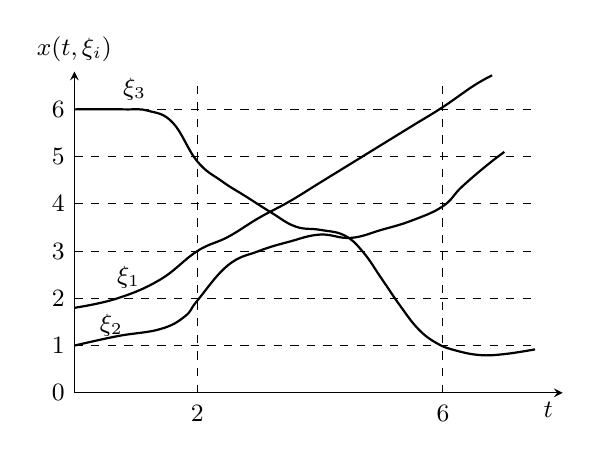
\begin{tikzpicture}[x=0.78cm,y=0.60cm,every node/.style={font=\small},>=stealth]
  \draw[->] (0,0) -- (7.95,0);
  \node[below left] at (7.95,0) {$t$};
  \draw[->] (0,0) -- (0,6.80);
  \node[above] at (0,6.80) {$x(t,\xi_i)$};
  % 水平虚线网格 y=1..6
  \foreach \y in {1,2,3,4,5,6}{%
    \draw[dashed] (0,\y) -- (7.55,\y);%
    \node[left] at (0,\y) {\y};}
  \node[left] at (0,0) {$0$};
  % t=2、t=6 处竖虚线
  \draw[dashed] (2,0) -- (2,6.65);
  \draw[dashed] (6,0) -- (6,6.65);
  \node[below] at (2,-0.06) {$2$};
  \node[below] at (6,-0.06) {$6$};
  % ξ3：起于 y=6，先平后降
  \draw[thick] plot[smooth,tension=0.7] coordinates {(0,6.00) (0.8,6.00) (1.2,5.97) (1.6,5.72) (2.0,4.90) (2.4,4.48) (2.8,4.15) (3.2,3.82) (3.6,3.52) (4.0,3.45) (4.4,3.33) (4.7,2.98) (5.0,2.42) (5.3,1.85) (5.6,1.35) (5.9,1.05) (6.2,0.90) (6.6,0.80) (7.0,0.82) (7.5,0.92)};
  % ξ1：起于 y≈1.8，单调上升
  \draw[thick] plot[smooth,tension=0.7] coordinates {(0,1.80) (0.7,2.00) (1.4,2.40) (2.0,3.00) (2.5,3.30) (3.0,3.70) (3.5,4.05) (4.0,4.45) (4.5,4.85) (5.0,5.25) (5.5,5.65) (6.0,6.05) (6.5,6.50) (6.8,6.72)};
  % ξ2：起于 y=1，先缓升后陡升
  \draw[thick] plot[smooth,tension=0.7] coordinates {(0,1.00) (0.7,1.20) (1.4,1.35) (1.8,1.62) (2.0,1.95) (2.5,2.70) (3.0,3.00) (3.5,3.20) (4.0,3.35) (4.5,3.28) (5.0,3.45) (5.5,3.65) (6.0,3.95) (6.3,4.35) (6.7,4.80) (7.0,5.10)};
  \node at (0.98,6.42) {$\xi_3$};
  \node at (0.88,2.45) {$\xi_1$};
  \node at (0.60,1.42) {$\xi_2$};
\end{tikzpicture}

\smallskip
{\small 图\,题2.2}
\end{center}

\exer{2.3}掷一枚硬币\nobreak，定义一个随机过程\nobreak：
\[
X(t)=\begin{cases}
\cos\pi t, & \text{出现正面}\\
2t, & \text{出现反面}
\end{cases}
\]
设“出现正面”和“出现反面”的概率相等\nobreak。试求\nobreak：

\begin{citemize}
\item （1\nobreak）$X(t)$ 的一维分布函数 $F_X(x,1/2)$\nobreak，$F_X(x,1)$\nobreak；
\item （2\nobreak）$X(t)$ 的二维分布函数 $F_X(x_1,x_2;1/2,1)$\nobreak；
\item （3\nobreak）画出上述分布函数的图形\nobreak。
\end{citemize}

\exer{2.4}假定二进制数据序列 $\{B(n),n=1,2,3,\cdots\}$ 是伯努利随机序列\nobreak，其每一位数据对应随机变量 $B(n)$\nobreak，并有概率 $P[B(n)=0]=0.2$ 和 $P[B(n)=1]=0.8$\nobreak。试求\nobreak：

\begin{citemize}
\item （1\nobreak）连续 4 位构成的串为 $\{1011\}$ 的概率是多少\nobreak？
\item （2\nobreak）连续 4 位构成的串的平均串是什么\nobreak？
\item （3\nobreak）连续 4 位构成的串中\nobreak，概率最大的是什么\nobreak？
\end{citemize}

\exer{2.5}正弦随机信号 $\{X(t,s)=A\cos(200\pi t),\ t>0\}$\nobreak，其中振幅随机变量 $A$ 取值为 1 和 0\nobreak，概率分别为 0.1 和 0.9\nobreak。试求\nobreak：

\begin{citemize}
\item （1\nobreak）一维概率分布 $F(x,5)$\nobreak；
\item （2\nobreak）二维概率分布 $F(x,y,0,0.0025)$\nobreak；
\item （3\nobreak）开启该设备后最可能见到什么样的信号\nobreak？
\item （4\nobreak）如果开启后 $t=1$ 时刻测得输出电压为 1~V\nobreak，问 $t=2$ 时刻可能的输出电压是什么\nobreak？概率是多少\nobreak？
\end{citemize}

\exer{2.6}若正弦信号 $X(t)=A\cos(\omega t+\Theta)$\nobreak，其中振幅 $A$ 与频率 $\omega$ 取常数\nobreak，相位 $\Theta$ 是一个随机变量\nobreak，它均匀分布于 $[-\pi,\pi]$ 间\nobreak，即
\[
f(\theta)=\begin{cases}
\dfrac{1}{2\pi}, & -\pi\leqslant\theta\leqslant\pi\\
0, & \text{其他}
\end{cases}
\]
求在 $t$ 时刻信号 $X(t)$ 的概率密度 $f_X(x)$\nobreak。

\exer{2.7}设质点运动的位置如直线过程 $X(t)=Vt+X_0$\nobreak，其中 $V\sim N(1,1)$\nobreak，$X_0\sim N(0,2)$\nobreak，并彼此独立\nobreak。试求 $t$ 时刻随机变量的一维概率密度函数\nobreak、均值与方差\nobreak。
% ↑ 「试求」在书 p.61 末行，句子后半截「$t$ 时刻随机变量的一维概率密度函数、均值与方差。」
%   是书 p.62 第一行，本片段按完整句子接排。

\exer{2.8}假定 $(-1,+1)$ 的伯努利序列 $\{I_n,n=1,2,\cdots\}$ 的取值具有等概特性\nobreak。试求它的一维概率密度函数\nobreak、均值与协方差函数\nobreak；

\exer{2.9}设某信号源每 $T$ 秒产生一个幅度为 $A$ 的方波脉冲\nobreak，其脉冲宽度 $X$ 为均匀分布于 $[0,T]$ 中的随机变量\nobreak。这样构成一个随机过程 $Y(t)$\nobreak，$0\leqslant t<\infty$\nobreak，其中一个样本函数如图题 2.9 所示\nobreak。设不同间隔中的脉冲宽度是统计独立的\nobreak，求 $Y(t)$ 的概率密度\nobreak。

\begin{center}
% 图题2.9：方波脉冲串 X1…X4（原书为手绘示意图）
% 读数（按扫描页标定）：脉冲起点分别在 t=0、T、2T、3T；
% 四个脉冲宽度约为 0.72T、0.40T、0.72T、0.84T，高度均为 A。
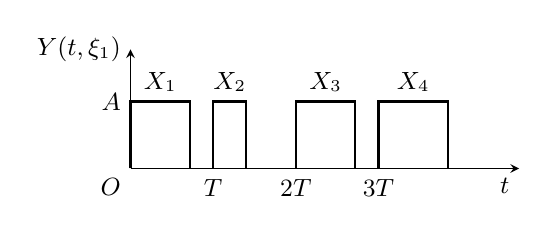
\begin{tikzpicture}[x=1.05cm,y=0.85cm,every node/.style={font=\small},>=stealth]
  \draw[->] (0,0) -- (4.70,0);
  \node[below left] at (4.70,0) {$t$};
  \draw[->] (0,0) -- (0,1.78);
  \node[left] at (0,1.78) {$Y(t,\xi_1)$};
  \node[left] at (0,1.00) {$A$};
  \node[below left] at (0,0) {$O$};
  \draw[thick] (0,0) -- (0,1) -- (0.72,1) -- (0.72,0);
  \draw[thick] (1,0) -- (1,1) -- (1.40,1) -- (1.40,0);
  \draw[thick] (2,0) -- (2,1) -- (2.72,1) -- (2.72,0);
  \draw[thick] (3,0) -- (3,1) -- (3.84,1) -- (3.84,0);
  \node[above] at (0.36,1.00) {$X_1$};
  \node[above] at (1.20,1.00) {$X_2$};
  \node[above] at (2.36,1.00) {$X_3$};
  \node[above] at (3.42,1.00) {$X_4$};
  \node[below] at (1,-0.02) {$T$};
  \node[below] at (2,-0.02) {$2T$};
  \node[below] at (3,-0.02) {$3T$};
\end{tikzpicture}

\smallskip
{\small 图\,题2.9}
\end{center}

\exer{2.10}给定随机过程 $X(t)$ 和常数 $a$\nobreak，试以 $X(t)$ 的自相关函数来表示差信号 $Y(t)=X(t+a)-X(t)$ 的自相关函数\nobreak。

\exer{2.11}两个随机信号 $X(t)=A\sin(\omega t+\Theta)$ 与 $Y(t)=B\cos(\omega t+\Theta)$\nobreak，其中 $A$ 与 $B$ 为未知随机变量\nobreak，$\Theta$ 为 $0\sim2\pi$ 内均匀分布的随机变量\nobreak，$A$\nobreak、$B$ 与 $\Theta$ 两两统计独立\nobreak，$\omega$ 为常数\nobreak。试求\nobreak：

\begin{citemize}
\item （1\nobreak）两个随机信号的互相关函数 $R_{XY}(t_1,t_2)$\nobreak；
\item （2\nobreak）讨论两个随机信号的正交性\nobreak、互不相关（无关\nobreak）与统计独立性\nobreak。
\end{citemize}

\exer{2.12}二项式随机信号 $Y(n)=\sum\limits_{i=1}^{n}X(i)$\nobreak，其中 $X(n)$ 是取值（0,1\nobreak）的伯努利随机信号\nobreak，$P[X(n)=0]=q$ 和 $P[X(n)=1]=p$\nobreak。试求\nobreak：

（1\nobreak）$Y(n)$ 的均值\nobreak；（2\nobreak）$\Var[Y(n)-Y(m)]$\nobreak，$n>m$\nobreak；（3\nobreak）$Y(n)$ 的相关函数\nobreak。

\exer{2.13}假定正弦电压信号 $X(t)=A\cos(\omega t+\Theta)$\nobreak，其中\nobreak，$\omega$ 为常数\nobreak，$A$ 服从均匀分布 $U(-1,+1)$\nobreak，$\Theta$ 服从均匀分布 $U(-\pi,+\pi)$\nobreak，它们彼此独立\nobreak。如果将信号施加到 RC 并联电路上\nobreak，求总的电流信号及其均方值\nobreak。

\exer{2.14}求随机信号的积分 $Y(t)=\int_0^t X(u)\dif u$ 的均值与相关函数表达式\nobreak。

\exer{2.15}高斯信号 $X(t)$ 的自相关函数为 $R_X(t_1-t_2)=0.5\eu^{-\lvert t_1-t_2\rvert}$\nobreak，均值为零\nobreak。求 $X(t)$ 的一维和二维概率密度\nobreak。

\exer{2.16}设随机过程 $X(t)=A\cos\omega t+B\sin\omega t$\nobreak，其中 $\omega$ 为常数\nobreak，$A$ 和 $B$ 是两个相互独立的高斯随机变量\nobreak。已知 $E[A]=E[B]=0$\nobreak，$E[A^2]=E[B^2]=\sigma^2$\nobreak，求 $X(t)$ 的一维和二维概率密度函数\nobreak。

\exer{2.17}设有零均值的高斯信号 $X(t)$\nobreak，令 $X_1=X(t_1)$\nobreak，$X_2=X(t_2)$\nobreak，$X_3=X(t_3)$ 和 $X_4=X(t_4)$\nobreak，试证明\nobreak：
\[
E[X_1X_2X_3X_4]=E[X_1X_2]E[X_3X_4]+E[X_1X_3]E[X_2X_4]+E[X_1X_4]E[X_2X_3]
\]

\exer{2.18}某高斯信号的均值 $m_X(t)=2$\nobreak，协方差 $C_X(t_1,t_2)=8\cos(t_1-t_2)$\nobreak，写出当 $t_1=0$\nobreak，$t_2=0.5$ 和 $t_3=1$ 时的三维概率密度\nobreak。

\exer{2.19}设随机变量 $(X,Y)\sim N(\bm{\mu},\bm{C})$\nobreak，其中 $\bm{\mu}=\begin{bmatrix}2\\2\end{bmatrix}$\nobreak，$\bm{C}=\begin{bmatrix}2&3\\3&5\end{bmatrix}$\nobreak，求 $(X,Y)$ 的概率密度和特征函数 $\phi_{XY}(u,v)$\nobreak。

\exer{2.20}若 $\bm{X}=(X_1,X_2,\cdots,X_n)^{\mathrm{T}}$ 是 $n$ 维（联合\nobreak）高斯随机变量\nobreak，试证明\nobreak：各随机变量相互独立的充要条件是两两互不相关\nobreak，即协方差矩阵为对角阵\nobreak，且对角线上的元素就是各个方差的值\nobreak。

\exer{2.21}计算机内存自地址 0 开始存放字节（8 位\nobreak）数据\nobreak，形成序列（假定高端地址值很大\nobreak）\nobreak，如果所有数据为随机\nobreak、彼此独立且同为均匀分布\nobreak。

\begin{citemize}
\item （1\nobreak）给出描述该数据序列的数学模型\nobreak；
\item （2\nobreak）求其相邻两字节为 0x55,0xAA 的概率\nobreak；
\item （3\nobreak）求其一维与二维概率特性\nobreak；
\item （4\nobreak）求其均值\nobreak、方差与协方差函数\nobreak。
\end{citemize}

% EQNUMBERS: （无）
% FIGNUMBERS: 图题2.2, 图题2.9（独立编号，不占 figure 计数器）
% PAGES: 61-62
% EXERCISES: 2.1 2.2 2.3 2.4 2.5 2.6 2.7 2.8 2.9 2.10 2.11 2.12 2.13
%            2.14 2.15 2.16 2.17 2.18 2.19 2.20 2.21（连续无跳号，末题 2.21，
%            其后即为书 p.62 页码「· 62 ·」，习题结束）

\end{document}
